% Options for packages loaded elsewhere
% Options for packages loaded elsewhere
\PassOptionsToPackage{unicode}{hyperref}
\PassOptionsToPackage{hyphens}{url}
%
\documentclass[
  11pt,
  letterpaper,
]{book}
\usepackage{xcolor}
\usepackage[margin=2.5cm,paper=a4paper]{geometry}
\usepackage{amsmath,amssymb}
\setcounter{secnumdepth}{5}
\usepackage{iftex}
\ifPDFTeX
  \usepackage[T1]{fontenc}
  \usepackage[utf8]{inputenc}
  \usepackage{textcomp} % provide euro and other symbols
\else % if luatex or xetex
  \usepackage{unicode-math} % this also loads fontspec
  \defaultfontfeatures{Scale=MatchLowercase}
  \defaultfontfeatures[\rmfamily]{Ligatures=TeX,Scale=1}
\fi
\usepackage{lmodern}
\ifPDFTeX\else
  % xetex/luatex font selection
\fi
% Use upquote if available, for straight quotes in verbatim environments
\IfFileExists{upquote.sty}{\usepackage{upquote}}{}
\IfFileExists{microtype.sty}{% use microtype if available
  \usepackage[]{microtype}
  \UseMicrotypeSet[protrusion]{basicmath} % disable protrusion for tt fonts
}{}
\makeatletter
\@ifundefined{KOMAClassName}{% if non-KOMA class
  \IfFileExists{parskip.sty}{%
    \usepackage{parskip}
  }{% else
    \setlength{\parindent}{0pt}
    \setlength{\parskip}{6pt plus 2pt minus 1pt}}
}{% if KOMA class
  \KOMAoptions{parskip=half}}
\makeatother
% Make \paragraph and \subparagraph free-standing
\makeatletter
\ifx\paragraph\undefined\else
  \let\oldparagraph\paragraph
  \renewcommand{\paragraph}{
    \@ifstar
      \xxxParagraphStar
      \xxxParagraphNoStar
  }
  \newcommand{\xxxParagraphStar}[1]{\oldparagraph*{#1}\mbox{}}
  \newcommand{\xxxParagraphNoStar}[1]{\oldparagraph{#1}\mbox{}}
\fi
\ifx\subparagraph\undefined\else
  \let\oldsubparagraph\subparagraph
  \renewcommand{\subparagraph}{
    \@ifstar
      \xxxSubParagraphStar
      \xxxSubParagraphNoStar
  }
  \newcommand{\xxxSubParagraphStar}[1]{\oldsubparagraph*{#1}\mbox{}}
  \newcommand{\xxxSubParagraphNoStar}[1]{\oldsubparagraph{#1}\mbox{}}
\fi
\makeatother
\usepackage{fancyvrb}

\usepackage{color}
\usepackage{fancyvrb}
\newcommand{\VerbBar}{|}
\newcommand{\VERB}{\Verb[commandchars=\\\{\}]}
\DefineVerbatimEnvironment{Highlighting}{Verbatim}{commandchars=\\\{\}}
% Add ',fontsize=\small' for more characters per line
\usepackage{framed}
\definecolor{shadecolor}{RGB}{241,243,245}
\newenvironment{Shaded}{\begin{snugshade}}{\end{snugshade}}
\newcommand{\AlertTok}[1]{\textcolor[rgb]{0.68,0.00,0.00}{#1}}
\newcommand{\AnnotationTok}[1]{\textcolor[rgb]{0.37,0.37,0.37}{#1}}
\newcommand{\AttributeTok}[1]{\textcolor[rgb]{0.40,0.45,0.13}{#1}}
\newcommand{\BaseNTok}[1]{\textcolor[rgb]{0.68,0.00,0.00}{#1}}
\newcommand{\BuiltInTok}[1]{\textcolor[rgb]{0.00,0.23,0.31}{#1}}
\newcommand{\CharTok}[1]{\textcolor[rgb]{0.13,0.47,0.30}{#1}}
\newcommand{\CommentTok}[1]{\textcolor[rgb]{0.37,0.37,0.37}{#1}}
\newcommand{\CommentVarTok}[1]{\textcolor[rgb]{0.37,0.37,0.37}{\textit{#1}}}
\newcommand{\ConstantTok}[1]{\textcolor[rgb]{0.56,0.35,0.01}{#1}}
\newcommand{\ControlFlowTok}[1]{\textcolor[rgb]{0.00,0.23,0.31}{\textbf{#1}}}
\newcommand{\DataTypeTok}[1]{\textcolor[rgb]{0.68,0.00,0.00}{#1}}
\newcommand{\DecValTok}[1]{\textcolor[rgb]{0.68,0.00,0.00}{#1}}
\newcommand{\DocumentationTok}[1]{\textcolor[rgb]{0.37,0.37,0.37}{\textit{#1}}}
\newcommand{\ErrorTok}[1]{\textcolor[rgb]{0.68,0.00,0.00}{#1}}
\newcommand{\ExtensionTok}[1]{\textcolor[rgb]{0.00,0.23,0.31}{#1}}
\newcommand{\FloatTok}[1]{\textcolor[rgb]{0.68,0.00,0.00}{#1}}
\newcommand{\FunctionTok}[1]{\textcolor[rgb]{0.28,0.35,0.67}{#1}}
\newcommand{\ImportTok}[1]{\textcolor[rgb]{0.00,0.46,0.62}{#1}}
\newcommand{\InformationTok}[1]{\textcolor[rgb]{0.37,0.37,0.37}{#1}}
\newcommand{\KeywordTok}[1]{\textcolor[rgb]{0.00,0.23,0.31}{\textbf{#1}}}
\newcommand{\NormalTok}[1]{\textcolor[rgb]{0.00,0.23,0.31}{#1}}
\newcommand{\OperatorTok}[1]{\textcolor[rgb]{0.37,0.37,0.37}{#1}}
\newcommand{\OtherTok}[1]{\textcolor[rgb]{0.00,0.23,0.31}{#1}}
\newcommand{\PreprocessorTok}[1]{\textcolor[rgb]{0.68,0.00,0.00}{#1}}
\newcommand{\RegionMarkerTok}[1]{\textcolor[rgb]{0.00,0.23,0.31}{#1}}
\newcommand{\SpecialCharTok}[1]{\textcolor[rgb]{0.37,0.37,0.37}{#1}}
\newcommand{\SpecialStringTok}[1]{\textcolor[rgb]{0.13,0.47,0.30}{#1}}
\newcommand{\StringTok}[1]{\textcolor[rgb]{0.13,0.47,0.30}{#1}}
\newcommand{\VariableTok}[1]{\textcolor[rgb]{0.07,0.07,0.07}{#1}}
\newcommand{\VerbatimStringTok}[1]{\textcolor[rgb]{0.13,0.47,0.30}{#1}}
\newcommand{\WarningTok}[1]{\textcolor[rgb]{0.37,0.37,0.37}{\textit{#1}}}

\usepackage{longtable,booktabs,array}
\usepackage{calc} % for calculating minipage widths
% Correct order of tables after \paragraph or \subparagraph
\usepackage{etoolbox}
\makeatletter
\patchcmd\longtable{\par}{\if@noskipsec\mbox{}\fi\par}{}{}
\makeatother
% Allow footnotes in longtable head/foot
\IfFileExists{footnotehyper.sty}{\usepackage{footnotehyper}}{\usepackage{footnote}}
\makesavenoteenv{longtable}
\usepackage{graphicx}
\makeatletter
\newsavebox\pandoc@box
\newcommand*\pandocbounded[1]{% scales image to fit in text height/width
  \sbox\pandoc@box{#1}%
  \Gscale@div\@tempa{\textheight}{\dimexpr\ht\pandoc@box+\dp\pandoc@box\relax}%
  \Gscale@div\@tempb{\linewidth}{\wd\pandoc@box}%
  \ifdim\@tempb\p@<\@tempa\p@\let\@tempa\@tempb\fi% select the smaller of both
  \ifdim\@tempa\p@<\p@\scalebox{\@tempa}{\usebox\pandoc@box}%
  \else\usebox{\pandoc@box}%
  \fi%
}
% Set default figure placement to htbp
\def\fps@figure{htbp}
\makeatother

\ifLuaTeX
  \usepackage{luacolor}
  \usepackage[soul]{lua-ul}
\else
  \usepackage{soul}
\fi




\setlength{\emergencystretch}{3em} % prevent overfull lines

\providecommand{\tightlist}{%
  \setlength{\itemsep}{0pt}\setlength{\parskip}{0pt}}



 
\usepackage[]{biblatex}
\addbibresource{ref/MAref.bib}


% AMTAIR Thesis Preamble - Zero package conflicts
% Only formatting commands, no package loading

% Line spacing for academic work
\usepackage{setspace}
\onehalfspacing

% Custom chapter formatting (remove "Chapter N" prefix) but unfortunately leaves blank space
\usepackage{titlesec}
\titleformat{\chapter}[display]
  {\normalfont\huge\bfseries}  % format
  {}                           % label (empty = no "Chapter N")
  {0pt}                        % sep
  {\Huge}                      % before-code



% Page formatting and headers
\usepackage{fancyhdr}
\pagestyle{fancy}
\fancyhf{}
\fancyhead[LE,RO]{\slshape\nouppercase{\rightmark}}
\fancyhead[LO,RE]{\slshape\nouppercase{\leftmark}}
\fancyfoot[C]{\thepage}

% % Fix page breaks after title page
% \newcommand{\cleartitlepage}{
%   \clearpage
%   \thispagestyle{empty}
%   \mbox{}
%   \clearpage
% }



\renewcommand{\maketitle}{}

%  Citation customization
% \usepackage[style=authoryear,backend=biber,natbib=true]{biblatex}

% % Custom citation commands for different contexts
% \newcommand{\citeauthor}[1]{\textcite{#1}}           % Author (year)
% \newcommand{\citeyear}[1]{(\citeyear*{#1})}         % (year)
% \newcommand{\citealt}[1]{\citeauthor{#1} \citeyear{#1}}  % Author year
% \newcommand{\citep}[1]{(\cite{#1})}                 # (Author, year)

% Page reference styling
% \DeclareFieldFormat{postnote}{#1}                    # No "p." prefix
% \DeclareFieldFormat{multipostnote}{#1}               # No "pp." prefix


% % Page numbering control
% \usepackage{afterpage}

% % Command to start front matter (roman numerals)
% \newcommand{\frontmatter}{
%   \cleardoublepage
%   \pagenumbering{roman}
%   \setcounter{page}{1}
% }

% % Command to start main matter (arabic numerals)
% \newcommand{\mainmatter}{
%   \cleardoublepage
%   \pagenumbering{arabic}
%   \setcounter{page}{1}
% }

% % Command to start back matter (continue arabic)
% \newcommand{\backmatter}{
%   \cleardoublepage
%   % Keep arabic numbering but could change style if needed
% }

% % Suppress page numbers on title page
% \newcommand{\titlepage}{
%   \thispagestyle{empty}
% }



% Commands for custom title page
% \newcommand{\thesistitle}{Automating the Modelling of Transformative Artificial Intelligence Risks}
% \newcommand{\thesisauthor}{Valentin Jakob Meyer}
\makeatletter
\@ifpackageloaded{tcolorbox}{}{\usepackage[skins,breakable]{tcolorbox}}
\@ifpackageloaded{fontawesome5}{}{\usepackage{fontawesome5}}
\definecolor{quarto-callout-color}{HTML}{909090}
\definecolor{quarto-callout-note-color}{HTML}{0758E5}
\definecolor{quarto-callout-important-color}{HTML}{CC1914}
\definecolor{quarto-callout-warning-color}{HTML}{EB9113}
\definecolor{quarto-callout-tip-color}{HTML}{00A047}
\definecolor{quarto-callout-caution-color}{HTML}{FC5300}
\definecolor{quarto-callout-color-frame}{HTML}{acacac}
\definecolor{quarto-callout-note-color-frame}{HTML}{4582ec}
\definecolor{quarto-callout-important-color-frame}{HTML}{d9534f}
\definecolor{quarto-callout-warning-color-frame}{HTML}{f0ad4e}
\definecolor{quarto-callout-tip-color-frame}{HTML}{02b875}
\definecolor{quarto-callout-caution-color-frame}{HTML}{fd7e14}
\makeatother
\makeatletter
\@ifpackageloaded{bookmark}{}{\usepackage{bookmark}}
\makeatother
\makeatletter
\@ifpackageloaded{caption}{}{\usepackage{caption}}
\AtBeginDocument{%
\ifdefined\contentsname
  \renewcommand*\contentsname{Table of contents}
\else
  \newcommand\contentsname{Table of contents}
\fi
\ifdefined\listfigurename
  \renewcommand*\listfigurename{List of Figures}
\else
  \newcommand\listfigurename{List of Figures}
\fi
\ifdefined\listtablename
  \renewcommand*\listtablename{List of Tables}
\else
  \newcommand\listtablename{List of Tables}
\fi
\ifdefined\figurename
  \renewcommand*\figurename{Figure}
\else
  \newcommand\figurename{Figure}
\fi
\ifdefined\tablename
  \renewcommand*\tablename{Table}
\else
  \newcommand\tablename{Table}
\fi
}
\@ifpackageloaded{float}{}{\usepackage{float}}
\floatstyle{ruled}
\@ifundefined{c@chapter}{\newfloat{codelisting}{h}{lop}}{\newfloat{codelisting}{h}{lop}[chapter]}
\floatname{codelisting}{Listing}
\newcommand*\listoflistings{\listof{codelisting}{List of Listings}}
\makeatother
\makeatletter
\usepackage{pdflscape}
\makeatother
\makeatletter
\makeatother
\makeatletter
\@ifpackageloaded{caption}{}{\usepackage{caption}}
\@ifpackageloaded{subcaption}{}{\usepackage{subcaption}}
\makeatother
\usepackage{bookmark}
\IfFileExists{xurl.sty}{\usepackage{xurl}}{} % add URL line breaks if available
\urlstyle{same}
\VerbatimFootnotes % allow verbatim text in footnotes
\hypersetup{
  pdftitle={Automating the Modelling of Transformative Artificial Intelligence Risks},
  pdfauthor={Valentin Jakob Meyer},
  hidelinks,
  pdfcreator={LaTeX via pandoc}}


\title{Automating the Modelling of Transformative Artificial
Intelligence Risks}
\usepackage{etoolbox}
\makeatletter
\providecommand{\subtitle}[1]{% add subtitle to \maketitle
  \apptocmd{\@title}{\par {\large #1 \par}}{}{}
}
\makeatother
\subtitle{An Epistemic Framework for Leveraging Frontier AI Systems to
Upscale Conditional Policy Assessments in Bayesian Networks on a Narrow
Path towards Existential Safety}
\author{Valentin Jakob Meyer}
\date{2025-05-26}
\begin{document}
\frontmatter
\maketitle

\begin{titlepage}
\thispagestyle{empty}% Remove page number from title page

% Top header with logo (left) and department (right)
\begin{minipage}{0.3\textwidth}
  
\includegraphics[width=5cm]{latex/uni-bayreuth-logo.png}
\end{minipage}
\hfill
\begin{minipage}{0.9\textwidth}
  \begin{center}
    -- P\&E Master's Programme --\\
    Chair of Philosophy, Computer\\
    Science \& Artificial Intelligence
  \end{center}
\end{minipage}

% Horizontal rule
\vspace{1.5cm}
\hrule
\vspace{2cm}

% Title in bold
\begin{center}
  \Large\textbf{Automating the Modelling of
Transformative Artificial Intelligence Risks}
\end{center}
\vspace{0.2cm}

\begin{center}
  -----
\end{center}
\vspace{0.2cm}

% Subtitle in italics with quotation marks
\begin{center}
  \normalsize``\textit{An Epistemic Framework for Leveraging Frontier AI Systems
to Upscale Conditional Policy Assessments in Bayesian Networks on a Narrow Path towards Existencial Safety }''
\end{center}
\vspace{0.2cm}

\begin{center}
  -----
\end{center}
\vspace{0.2cm}

% Thesis designation
\begin{center}
  A thesis submitted at the Department of Philosophy\\[0.4cm]
  for the degree of \textit{Master of Arts in Philosophy \& Economics}
\end{center}

\vspace{1.5cm}
% Horizontal rule
\hrule
\vspace{1.5cm}

% Author and supervisor information with precise alignment
\begin{minipage}[t]{0.48\textwidth}
  \textbf{Author:}\\[0.3cm]
  \href{https://www.vjmeyer.org}{Valentin Jakob Meyer}\\
  \href{mailto:Valentin.meyer@uni-bayreuth.de}{Valentin.meyer@uni-bayreuth.de}\\
  \textit{Matriculation Number:} 1828610\\
  \textit{Tel.:} +49 (1573) 4512494\\
  Pielmühler Straße 15\\
  52066 Lappersdorf
\end{minipage}
\hfill
\begin{minipage}[t]{0.48\textwidth}
  \begin{flushright}
    \textbf{Supervisor:}\\[0.3cm]
    \href{mailto:timo.speith@uni-bayreuth.de}{Dr. Timo Speith}\\[0.35cm]
    \textit{Word Count:}\\
    30.000\\[0.1cm]
    \textit{Source / Identifier:}\\
    \href{https://github.com/VJMeyer/submission}{Document URL}
  \end{flushright}
\end{minipage}

% Date at bottom
\vfill
\begin{center}
  26th of May 2025
\end{center}
\end{titlepage}

% Critical: Clean page break to TOC
\cleardoublepage

\renewcommand*\contentsname{Table of Contents}
{
\setcounter{tocdepth}{2}
\tableofcontents
}
\listoffigures
\listoftables

\mainmatter
\bookmarksetup{startatroot}

\chapter*{Preface}\label{preface}
\addcontentsline{toc}{chapter}{Preface}

\markboth{Preface}{Preface}

\bookmarksetup{startatroot}

\chapter*{Quarto Syntax}\label{sec-syntax}
\addcontentsline{toc}{chapter}{Quarto Syntax}

\markboth{Quarto Syntax}{Quarto Syntax}

\section*{Main Formatting}\label{main-formatting}
\addcontentsline{toc}{section}{Main Formatting}

\markright{Main Formatting}

\subsection*{Html Comments}\label{html-comments}
\addcontentsline{toc}{subsection}{Html Comments}

\section*{Syntax for Tasks}\label{syntax-for-tasks}
\addcontentsline{toc}{section}{Syntax for Tasks}

\markright{Syntax for Tasks}

\subsection*{Tasks with ToDo Tree}\label{tasks-with-todo-tree}
\addcontentsline{toc}{subsection}{Tasks with ToDo Tree}

\subsubsection*{Simple ``One-line tasks''}\label{simple-one-line-tasks}
\addcontentsline{toc}{subsubsection}{Simple ``One-line tasks''}

Use Code ticks and html comment and task format for tasks distinctly
visible across all formats including the ToDo-Tree overview:

\texttt{\textless{}!-\/-\ {[}\ {]}\ ToDos\ for\ things\ to\ do\ /\ tasks\ /\ reminders\ (allows\ "jump\ to\ with\ Taks\ Tree\ extension")\ -\/-\textgreater{}}

Use html comment and task format for open or uncertain tasks, visible in
the .qmd file:

\subsubsection*{More Complex Tasks with
Notes}\label{more-complex-tasks-with-notes}
\addcontentsline{toc}{subsubsection}{More Complex Tasks with Notes}

\begin{verbatim}
<!-- [ ] Task Title: short description-->

  More Information about task

  Relevant notes

  Step-by-step implementation Plan

  Etc.
\end{verbatim}

\subsubsection*{Completed Tasks}\label{completed-tasks}
\addcontentsline{toc}{subsubsection}{Completed Tasks}

Retain completed tasks in ToDo-Tree by adding an x in the brackets:
\texttt{{[}x{]}}
\texttt{\textless{}!-\/-\ {[}x{]}\ Tasks\ which\ have\ been\ finished\ but\ should\ remain\ for\ later\ verification\ -\/-\textgreater{}}

Mark and remove completed tasks from ToDo-Tree by adding a minus in the
brackets: \texttt{{[}-{]}}

\texttt{\textless{}!-\/-\ {[}-{]}\ Tasks\ which\ have\ been\ finished\ but\ should\ remain\ visible\ for\ later\ verification\ -\/-\textgreater{}}

\subsubsection*{Missing Citations}\label{missing-citations}
\addcontentsline{toc}{subsubsection}{Missing Citations}

\texttt{\textless{}!-\/-\ {[}\ {]}\ FIND:\ @CITATION\_KEY\_PURPOSE:\ "Description\ of\ the\ appropriate/idea\ source,\ including\ ideas\ /suggestions\ /\ search\ terms\ etc."\ -\/-\textgreater{}}

\subsubsection*{Suggested Citation}\label{suggested-citation}
\addcontentsline{toc}{subsubsection}{Suggested Citation}

\texttt{\textless{}!-\/-\ {[}\ {]}\ VERIFY:\ @CITATION\_KEY\_SUGGESTED:\ "Description\ of\ the\ appropriate\ paper,\ book,\ source"\ {[}Include\ BibTex\ if\ known{]}\ -\/-\textgreater{}}

\subsubsection*{Missing Graphic}\label{missing-graphic}
\addcontentsline{toc}{subsubsection}{Missing Graphic}

\texttt{\textless{}!-\/-\ {[}\ {]}\ FIND:\ \{\#fig-GRAPHIC\_IDEA\}{]}:\ "Description\ of\ the\ appropriate/idea\ source,\ including\ ideas\ /suggestions\ /\ search\ terms\ etc."\ -\/-\textgreater{}}

\subsubsection*{Suggested Graphic}\label{suggested-graphic}
\addcontentsline{toc}{subsubsection}{Suggested Graphic}

\texttt{\textless{}!-\/-\ {[}\ {]}\ VERIFY:\ \{\#fig-GRAPHIC\_IDEA\}:\ "Description\ of\ the\ appropriate\ paper,\ book,\ source"\ {[}Include\ figure\ syntax\ if\ known{]}\ -\/-\textgreater{}}

Missing and/or suggested tables, concepts, explanations as well as other
elements should be suggested similarily.

\subsection*{Task Syntax Examples}\label{task-syntax-examples}
\addcontentsline{toc}{subsection}{Task Syntax Examples}

\texttt{\textless{}!-\/-\ {[}\ {]}\ (Example\ short:\ open\ and\ visible\ in\ text)\ \ \ Find\ and\ list\ the\ names\ of\ the\ MTAIR\ team-members\ responsible\ for\ the\ Analytica\ Implementation\ -\/-\textgreater{}}

\begin{verbatim}
<!-- [ ] (Example longer: open and visible in text)    Review/Plan/Discuss integrating Live Prediction Markets -->

  Live prediction market integration requires:
    (1) API connections to platforms (Metaculus, Manifold),
    (2) Question-to-variable mapping algorithms,
    (3) Probability update mechanisms, 
    (4) Handling of market dynamics (thin markets, manipulation).
    Current mentions may overstate readiness or underestimate complexity.
    Need realistic assessment of what's achievable.

  Implementation Steps:
      0. List/mention all relevant platforms with a brief description each
      1. Review all existing prediction market mentions for accuracy
      2. Assess actual API availability and limitations
      3. Describe/explain/discuss how to implement basic proof-of-concept with single platform
      4. Document challenges: question mapping, market interpretation
      5. Create realistic timeline for full implementation
      6. Revise thesis claims to match reality
      7. Add "Future Work" and/or extension section on complete integration
      8. Include descriptions of mockups/designs even if not fully built 
      9. Highlight/discuss the advantages of such integrations
      10. Quickly brainstorm for downsides worth mentioning
\end{verbatim}

\subsection*{Verbatim Code Formatting}\label{verbatim-code-formatting}
\addcontentsline{toc}{subsection}{Verbatim Code Formatting}

\texttt{verbatim\ code\ formatting\ for\ notes\ and\ ideas\ to\ be\ included\ (here)}

\subsection*{Code Block formatting}\label{code-block-formatting}
\addcontentsline{toc}{subsection}{Code Block formatting}

\begin{verbatim}
Also code blocks for more extensive notes and ideas to be included and checklists
- test 1. 
- test 2. 
- test 3.
2. second
3. third
\end{verbatim}

\begin{verbatim}
code
\end{verbatim}

Add a language to syntax highlight code blocks:

\begin{Shaded}
\begin{Highlighting}[]
\DecValTok{1} \OperatorTok{+} \DecValTok{1}
\end{Highlighting}
\end{Shaded}

\subsection*{Blockquote Formatting}\label{blockquote-formatting}
\addcontentsline{toc}{subsection}{Blockquote Formatting}

\begin{quote}
Blockquote formatting for ``Suggested Citations (e.g.~carlsmith 2024 on
\ldots)'' and/or claims which require a citation (e.g.~claim x should be
backed-up by a ciation from the literature)
\end{quote}

\subsection*{Tables}\label{tables}
\addcontentsline{toc}{subsection}{Tables}

\begin{longtable}[]{@{}rllc@{}}
\caption{Demonstration of pipe table
syntax}\label{tbl-letters}\tabularnewline
\toprule\noalign{}
Right & Left & Default & Center \\
\midrule\noalign{}
\endfirsthead
\toprule\noalign{}
Right & Left & Default & Center \\
\midrule\noalign{}
\endhead
\bottomrule\noalign{}
\endlastfoot
12 & 12 & 12 & 12 \\
123 & 123 & 123 & 123 \\
1 & 1 & 1 & 1 \\
\end{longtable}

\begin{longtable}[]{@{}lll@{}}
\caption{My Caption 1}\label{tbl-letters}\tabularnewline
\toprule\noalign{}
Col1 & Col2 & Col3 \\
\midrule\noalign{}
\endfirsthead
\toprule\noalign{}
Col1 & Col2 & Col3 \\
\midrule\noalign{}
\endhead
\bottomrule\noalign{}
\endlastfoot
A & B & C \\
E & F & G \\
A & G & G \\
\end{longtable}

Referencing tables with \texttt{@tbl-KEY}: See Table~\ref{tbl-letters}.

\begin{table}

\caption{\label{tbl-panel}Main Caption}

\begin{minipage}{0.50\linewidth}

\subcaption{\label{tbl-first}First Table}

\centering{

\begin{tabular}{lll}
\toprule
Col1 & Col2 & Col3\\
\midrule
A & B & C\\
E & F & G\\
A & G & G\\
\bottomrule
\end{tabular}

}

\end{minipage}%
%
\begin{minipage}{0.50\linewidth}

\subcaption{\label{tbl-second}Second Table}

\centering{

\begin{tabular}{lll}
\toprule
Col1 & Col2 & Col3\\
\midrule
A & B & C\\
E & F & G\\
A & G & G\\
\bottomrule
\end{tabular}

}

\end{minipage}%

\end{table}%

See Table~\ref{tbl-panel} for details, especially
Table~\ref{tbl-second}.

\begin{Shaded}
\begin{Highlighting}[]
\NormalTok{python}
\NormalTok{\#| label: tbl{-}planets}
\NormalTok{\#| tbl{-}cap: Astronomical object}

\NormalTok{from IPython.display import Markdown}
\NormalTok{from tabulate import tabulate}
\NormalTok{table = [}\CommentTok{[}\OtherTok{"Sun","696,000",1.989e30}\CommentTok{]}\NormalTok{,}
         \CommentTok{[}\OtherTok{"Earth","6,371",5.972e24}\CommentTok{]}\NormalTok{,}
         \CommentTok{[}\OtherTok{"Moon","1,737",7.34e22}\CommentTok{]}\NormalTok{,}
         \CommentTok{[}\OtherTok{"Mars","3,390",6.39e23}\CommentTok{]}\NormalTok{]}
\NormalTok{Markdown(tabulate(}
\NormalTok{  table, }
\NormalTok{  headers=}\CommentTok{[}\OtherTok{"Astronomical object","R (km)", "mass (kg)"}\CommentTok{]}
\NormalTok{))}
\end{Highlighting}
\end{Shaded}

\begin{longtable}[]{@{}
  >{\raggedright\arraybackslash}p{(\linewidth - 4\tabcolsep) * \real{0.1806}}
  >{\raggedright\arraybackslash}p{(\linewidth - 4\tabcolsep) * \real{0.1806}}
  >{\raggedright\arraybackslash}p{(\linewidth - 4\tabcolsep) * \real{0.3194}}@{}}
\caption{Sample grid table.}\tabularnewline
\toprule\noalign{}
\begin{minipage}[b]{\linewidth}\raggedright
Fruit
\end{minipage} & \begin{minipage}[b]{\linewidth}\raggedright
Price
\end{minipage} & \begin{minipage}[b]{\linewidth}\raggedright
Advantages
\end{minipage} \\
\midrule\noalign{}
\endfirsthead
\toprule\noalign{}
\begin{minipage}[b]{\linewidth}\raggedright
Fruit
\end{minipage} & \begin{minipage}[b]{\linewidth}\raggedright
Price
\end{minipage} & \begin{minipage}[b]{\linewidth}\raggedright
Advantages
\end{minipage} \\
\midrule\noalign{}
\endhead
\bottomrule\noalign{}
\endlastfoot
Bananas & \$1.34 & \begin{minipage}[t]{\linewidth}\raggedright
\begin{itemize}
\tightlist
\item
  built-in wrapper
\item
  bright color
\end{itemize}
\end{minipage} \\
Oranges & \$2.10 & \begin{minipage}[t]{\linewidth}\raggedright
\begin{itemize}
\tightlist
\item
  cures scurvy
\item
  tasty
\end{itemize}
\end{minipage} \\
\end{longtable}

Content with HTML tables you don't want processed.

\section*{Headings \& Potential Headings in Standard Markdown formatting
(`\#\#')}\label{sec-heading}
\addcontentsline{toc}{section}{Headings \& Potential Headings in
Standard Markdown formatting (`\#\#')}

\markright{Headings \& Potential Headings in Standard Markdown
formatting (`\#\#')}

\subsection*{Heading 3}\label{heading-3}
\addcontentsline{toc}{subsection}{Heading 3}

\subsubsection*{Heading 4}\label{heading-4}
\addcontentsline{toc}{subsubsection}{Heading 4}

\section*{Text Formatting Options}\label{text-formatting-options}
\addcontentsline{toc}{section}{Text Formatting Options}

\markright{Text Formatting Options}

\emph{italics}, \textbf{bold}, \textbf{\emph{bold italics}}

superscript\textsuperscript{2} and subscript\textsubscript{2}

\st{strikethrough}

\hl{This text is highlighted}

\ul{This text is underlined}

\textsc{This text is smallcaps}

\section*{Lists}\label{lists}
\addcontentsline{toc}{section}{Lists}

\markright{Lists}

\begin{itemize}
\item
  unordered list

  \begin{itemize}
  \tightlist
  \item
    sub-item 1
  \item
    sub-item 2

    \begin{itemize}
    \tightlist
    \item
      sub-sub-item 1
    \end{itemize}
  \end{itemize}
\item
  item 2

  Continued (indent 4 spaces)
\end{itemize}

\begin{enumerate}
\def\labelenumi{\arabic{enumi}.}
\tightlist
\item
  ordered list
\item
  item 2

  \begin{enumerate}
  \def\labelenumii{\roman{enumii})}
  \tightlist
  \item
    sub-item 1

    \begin{enumerate}
    \def\labelenumiii{\Alph{enumiii}.}
    \tightlist
    \item
      sub-sub-item 1
    \end{enumerate}
  \end{enumerate}
\end{enumerate}

\section*{Math}\label{math}
\addcontentsline{toc}{section}{Math}

\markright{Math}

inline math: \(E = mc^{2}\)

display math:

\[E = mc^{2}\]

If you want to define custom TeX macros, include them within \$\$
delimiters enclosed in a .hidden block. For example:

\[
 \def\RR{{\bf R}}
 \def\bold#1{{\bf #1}}
\]

For HTML math processed using MathJax (the default) you can use the
\textbackslash def, \textbackslash newcommand,
\textbackslash renewcommand, \textbackslash newenvironment,
\textbackslash renewenvironment, and \textbackslash let commands to
create your own macros and environments.

\section*{Footnotes}\label{footnotes}
\addcontentsline{toc}{section}{Footnotes}

\markright{Footnotes}

Here is an inline note.\footnote{Inlines notes are easier to write,
  since you don't have to pick an identifier and move down to type the
  note.}

Here is a footnote reference,\footnote{Here is the footnote.}

Another Text with a footnote\footnote{Here's one with multiple blocks.

  Subsequent paragraphs are indented to show that they belong to the
  previous footnote.

\begin{Verbatim}
{ some.code }
\end{Verbatim}

  The whole paragraph can be indented, or just the first line. In this
  way, multi-paragraph footnotes work like multi-paragraph list items.}
but this time a ``longnote''.

This paragraph won't be part of the note, because it isn't indented.

\section*{Callouts}\label{sec-callouts}
\addcontentsline{toc}{section}{Callouts}

\markright{Callouts}

Quarto's native callouts work without additional packages:

This is written in a `note' environment -- but it does not seem to
produce any special rendering.

\begin{tcolorbox}[enhanced jigsaw, title=\textcolor{quarto-callout-note-color}{\faInfo}\hspace{0.5em}{Optional Title}, breakable, colbacktitle=quarto-callout-note-color!10!white, opacityback=0, opacitybacktitle=0.6, coltitle=black, bottomtitle=1mm, colback=white, arc=.35mm, toptitle=1mm, colframe=quarto-callout-note-color-frame, titlerule=0mm, rightrule=.15mm, bottomrule=.15mm, left=2mm, leftrule=.75mm, toprule=.15mm]

Content here

\end{tcolorbox}

\begin{tcolorbox}[enhanced jigsaw, title=\textcolor{quarto-callout-note-color}{\faInfo}\hspace{0.5em}{Important Note2}, breakable, colbacktitle=quarto-callout-note-color!10!white, opacityback=0, opacitybacktitle=0.6, coltitle=black, bottomtitle=1mm, colback=white, arc=.35mm, toptitle=1mm, colframe=quarto-callout-note-color-frame, titlerule=0mm, rightrule=.15mm, bottomrule=.15mm, left=2mm, leftrule=.75mm, toprule=.15mm]

This renders perfectly in both HTML and PDF.

\end{tcolorbox}

Also for markdown:

\begin{Shaded}
\begin{Highlighting}[]
\NormalTok{::: \{.render\_as\_markdown\_example\}}
\FunctionTok{\#\# Markdown Heading}
\NormalTok{This renders perfectly in both HTML and PDF but as markdown "plain text"}
\NormalTok{:::}
\end{Highlighting}
\end{Shaded}

\section*{Links}\label{links}
\addcontentsline{toc}{section}{Links}

\markright{Links}

\texttt{\textless{}https://quarto.org/docs/authoring/markdown-basics.html\textgreater{}}
produces: \url{https://quarto.org/docs/authoring/markdown-basics.html}

\texttt{{[}Quarto\ Book\ Cross-References{]}(https://quarto.org/docs/books/book-crossrefs.html)}
produces:
\href{https://quarto.org/docs/books/book-crossrefs.html}{Quarto Book
Cross-References}

\section*{Images \& Figures}\label{sec-figures1}

\markright{Images \& Figures}

\begin{verbatim}
[![AMTAIR Automation Pipeline from @bucknall2022](/images/pipeline.png){
  #fig-automation_pipeline
  fig-scap="Five-step AMTAIR automation pipeline from PDFs to Bayesian networks" 
  fig-alt="FLOWCHART: Five-step automation pipeline workflow for AMTAIR project.
          DATA: The pipeline transforms PDFs through ArgDown, BayesDown, CSV, and HTML into Bayesian network visualizations.
          PURPOSE: Illustrates the core technical process that enables automated extraction of probabilistic models from AI safety literature.
          DETAILS: Five numbered green steps show: (1) LLM-based extraction from PDFs to ArgDown, (2) ArgDown to BayesDown completion with probabilities, (3) Extracting world-models as CSV data, (4) Software tools for data inference, and (5) Visualization of the resulting Bayesian network.
          Each step includes example outputs, with the final visualization showing a Rain-Sprinkler-Grass Wet Bayesian network with probability tables.
          SOURCE: Created by the author to explain the AMTAIR methodology
          "
  fig-align="center" 
  width="100%"
  }](https://github.com/VJMeyer/submission)


Testing crossreferencing grapics @fig-automation_pipeline.

![Caption/Title 2](/images/cover.png){#fig-testgraphic2 fig-scap="Short 2 caption" fig-alt="2nd Alt Text / Description." fig-align="left" width="30%"}

Testing crossreferencing grapics @fig-testgraphic2.
\end{verbatim}

\begin{figure}

\centering{

\href{https://github.com/VJMeyer/submission}{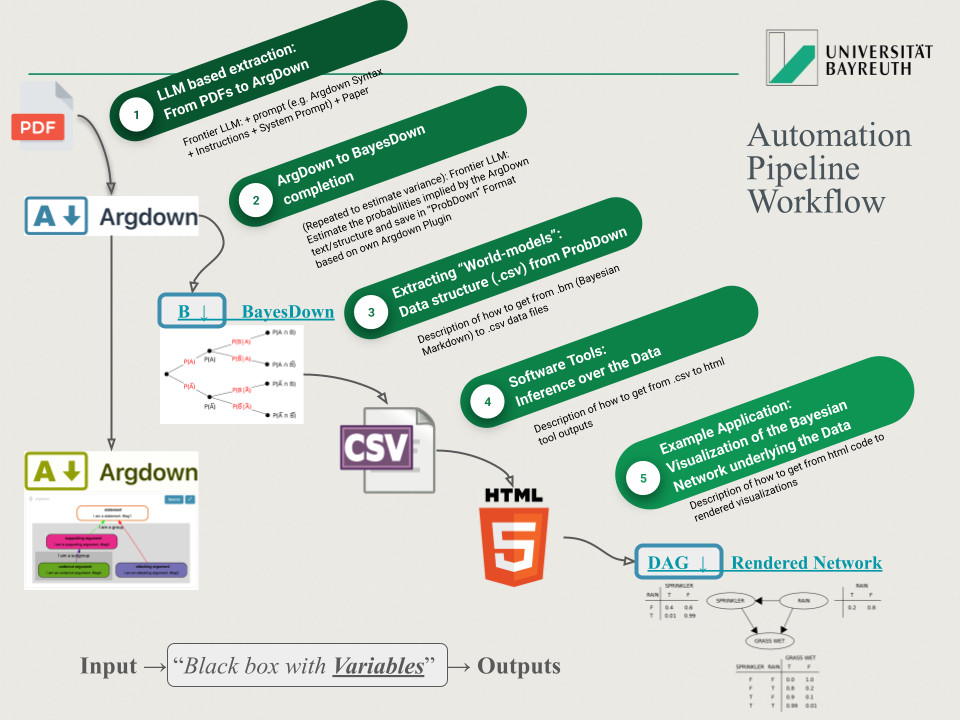
\includegraphics[width=1\linewidth,height=\textheight,keepaspectratio]{images/pipeline.png}}

}

\caption[Five-step AMTAIR automation pipeline from PDFs to Bayesian
networks]{\label{fig-automation_pipeline}AMTAIR Automation Pipeline
from}

\end{figure}%

Testing crossreferencing grapics Figure~\ref{fig-automation_pipeline}.
Note that the indentations of graphic inclusions get messed up by
viewing them in ``view mode'' in VS code.

\begin{figure}


\includegraphics[width=0.3\linewidth,height=\textheight,keepaspectratio]{images/cover.png}

\caption[Short 2 caption]{\label{fig-testgraphic2}Caption/Title 2}

\end{figure}%

Testing crossreferencing grapics Figure~\ref{fig-testgraphic2}.

\section*{Page Breaks}\label{page-breaks}
\addcontentsline{toc}{section}{Page Breaks}

\markright{Page Breaks}

\begin{Shaded}
\begin{Highlighting}[]
\NormalTok{page 1}



\NormalTok{page 2}
\end{Highlighting}
\end{Shaded}

page 1

\newpage{}

page 2

\section*{Including Code}\label{sec-code}
\addcontentsline{toc}{section}{Including Code}

\markright{Including Code}

\begin{figure}

\centering{

\begin{Shaded}
\begin{Highlighting}[]
\ImportTok{import}\NormalTok{ pandas }\ImportTok{as}\NormalTok{ pd}
\BuiltInTok{print}\NormalTok{(}\StringTok{"AMTAIR is working!"}\NormalTok{)}
\end{Highlighting}
\end{Shaded}

\begin{verbatim}
AMTAIR is working!
\end{verbatim}

}

\caption{\label{fig-extraction-pipeline}}

\end{figure}%

\subsection*{In-Line LaTeX}\label{in-line-latex}
\addcontentsline{toc}{subsection}{In-Line LaTeX}

\renewcommand*{\labelitemi}{\textgreater}

\subsection*{In-Line HTML}\label{in-line-html}
\addcontentsline{toc}{subsection}{In-Line HTML}

Here's some raw inline HTML: html

\section*{Reference or Embed Code from .ipynb
files}\label{reference-or-embed-code-from-.ipynb-files}
\addcontentsline{toc}{section}{Reference or Embed Code from .ipynb
files}

\markright{Reference or Embed Code from .ipynb files}

\subsubsection*{Code chunks from .ipynb notebooks can be embedded in the
.qmd text
with:}\label{code-chunks-from-.ipynb-notebooks-can-be-embedded-in-the-.qmd-text-with}
\addcontentsline{toc}{subsubsection}{Code chunks from .ipynb notebooks
can be embedded in the .qmd text with:}

\begin{Shaded}
\begin{Highlighting}[]
\NormalTok{\{\{\textless{} embed /AMTAIR\_Prototype/data/example\_carlsmith/AMTAIR\_Prototype\_example\_carlsmith.ipynb\#my\_code\_cell\_test \textgreater{}\}\}}
\end{Highlighting}
\end{Shaded}

\subsubsection*{which produces the output of executing the code
cell:}\label{which-produces-the-output-of-executing-the-code-cell}
\addcontentsline{toc}{subsubsection}{which produces the output of
executing the code cell:}

\phantomsection\label{my_code_cell_test}
\begin{verbatim}
Connecting to repository: https://raw.githubusercontent.com/SingularitySmith/AMTAIR_Prototype/main/data/example_carlsmith/
Attempting to load: https://raw.githubusercontent.com/SingularitySmith/AMTAIR_Prototype/main/data/example_carlsmith/ArgDown.md
✅ Successfully connected to repository and loaded test files.
[Existential_Catastrophe]: The destruction of humanity's long-term potential due to AI systems we've lost control over. {"instantiations": ["existential_catastrophe_TRUE", "existential_catastrophe_FALSE"]}
- [Human_Disempowerment]: Permanent and collective disempowerment of humanity relative to AI systems. {"instantiations": ["human_disempowerment_TRUE", "human_disempowerment_FALSE"]}
    - [Scale_Of_Power_Seeking]: Power-seeking by AI systems scaling to the point of permanently disempowering all of humanity. {"instantiations": ["scale_of_power_seeking_TRUE", "scale_of_power_seeking_FALSE"]}
        - [Misaligned_Power_Seeking]: Deployed AI systems seeking power in unintended and high-impact ways due to problems with their objectives. {"instantiations": ["misaligned_power_seeking_TRUE", "misaligned_power_seeking_FALSE"]}
            - [APS_Systems]: AI systems with advanced capabilities, agentic planning, and strategic awareness. {"instantiations": ["aps_systems_TRUE", "aps_systems_FALSE"]}
                - [Advanced_AI_Capability]: AI systems that outperform humans on tasks that grant significant power in the world. {"instantiations": ["advanced_ai_capability_TRUE", "advanced_ai_capability_FALSE"]}
                - [Agentic_Planning]: AI systems making and executing plans based on world models to achieve objectives. {"instantiations": ["agentic_planning_TRUE", "agentic_planning_FALSE"]}
                - [Strategic_Awareness]: AI systems with models accurately representing power dynamics with humans. {"instantiations": ["strategic_awareness_TRUE", "strategic_awareness_FALSE"]}
            - [Difficulty_Of_Alignment]: It is harder to build aligned systems than misaligned systems that are attractive to deploy. {"instantiations": ["difficulty_of_alignment_TRUE", "difficulty_of_alignment_FALSE"]}
                - [Instrumental_Convergence]: AI systems with misaligned objectives tend to seek power as an instrumental goal. {"instantiations": ["instrumental_convergence_TRUE", "instrumental_convergence_FALSE"]}
                - [Problems_With_Proxies]: Optimizing for proxy objectives breaks correlations with intended goals. {"instantiations": ["problems_with_proxies_TRUE", "problems_with_proxies_FALSE"]}
                - [Problems_With_Search]: Search processes can yield systems pursuing different objectives than intended. {"instantiations": ["problems_with_search_TRUE", "problems_with_search_FALSE"]}
            - [Deployment_Decisions]: Decisions to deploy potentially misaligned AI systems. {"instantiations": ["deployment_decisions_DEPLOY", "deployment_decisions_WITHHOLD"]}
                - [Incentives_To_Build_APS]: Strong incentives to build and deploy APS systems. {"instantiations": ["incentives_to_build_aps_STRONG", "incentives_to_build_aps_WEAK"]}
                    - [Usefulness_Of_APS]: APS systems are very useful for many valuable tasks. {"instantiations": ["usefulness_of_aps_HIGH", "usefulness_of_aps_LOW"]}
                    - [Competitive_Dynamics]: Competitive pressures between AI developers. {"instantiations": ["competitive_dynamics_STRONG", "competitive_dynamics_WEAK"]}
                - [Deception_By_AI]: AI systems deceiving humans about their true objectives. {"instantiations": ["deception_by_ai_TRUE", "deception_by_ai_FALSE"]}
        - [Corrective_Feedback]: Human society implementing corrections after observing problems. {"instantiations": ["corrective_feedback_EFFECTIVE", "corrective_feedback_INEFFECTIVE"]}
            - [Warning_Shots]: Observable failures in weaker systems before catastrophic risks. {"instantiations": ["warning_shots_OBSERVED", "warning_shots_UNOBSERVED"]}
            - [Rapid_Capability_Escalation]: AI capabilities escalating very rapidly, allowing little time for correction. {"instantiations": ["rapid_capability_escalation_TRUE", "rapid_capability_escalation_FALSE"]}
[Barriers_To_Understanding]: Difficulty in understanding the internal workings of advanced AI systems. {"instantiations": ["barriers_to_understanding_HIGH", "barriers_to_understanding_LOW"]}
- [Misaligned_Power_Seeking]: Deployed AI systems seeking power in unintended and high-impact ways due to problems with their objectives. {"instantiations": ["misaligned_power_seeking_TRUE", "misaligned_power_seeking_FALSE"]}
[Adversarial_Dynamics]: Potentially adversarial relationships between humans and power-seeking AI. {"instantiations": ["adversarial_dynamics_TRUE", "adversarial_dynamics_FALSE"]}
- [Misaligned_Power_Seeking]: Deployed AI systems seeking power in unintended and high-impact ways due to problems with their objectives. {"instantiations": ["misaligned_power_seeking_TRUE", "misaligned_power_seeking_FALSE"]}
[Stakes_Of_Error]: The escalating impact of mistakes with power-seeking AI systems. {"instantiations": ["stakes_of_error_HIGH", "stakes_of_error_LOW"]}
- [Misaligned_Power_Seeking]: Deployed AI systems seeking power in unintended and high-impact ways due to problems with their objectives. {"instantiations": ["misaligned_power_seeking_TRUE", "misaligned_power_seeking_FALSE"]}
\end{verbatim}

\subsubsection*{including `echo=true' renders the code of the
cell:}\label{including-echotrue-renders-the-code-of-the-cell}
\addcontentsline{toc}{subsubsection}{including `echo=true' renders the
code of the cell:}

\begin{Shaded}
\begin{Highlighting}[]
\NormalTok{\{\{\textless{} embed /AMTAIR\_Prototype/data/example\_carlsmith/AMTAIR\_Prototype\_example\_carlsmith.ipynb\#my\_code\_cell\_test echo=true \textgreater{}\}\}}
\end{Highlighting}
\end{Shaded}

\phantomsection\label{my_code_cell_test}
\begin{Shaded}
\begin{Highlighting}[]
\CommentTok{\# @title 0.2 {-}{-}{-} Connect to GitHub Repository {-}{-}{-} Load Files}

\CommentTok{"""}
\CommentTok{BLOCK PURPOSE: Establishes connection to the AMTAIR GitHub repository and provides}
\CommentTok{functions to load example data files for processing.}

\CommentTok{This block creates a reusable function for accessing files from the project\textquotesingle{}s}
\CommentTok{GitHub repository, enabling access to example files like the rain{-}sprinkler{-}lawn}
\CommentTok{Bayesian network that serves as our canonical test case.}

\CommentTok{DEPENDENCIES: requests library, io library}
\CommentTok{OUTPUTS: load\_file\_from\_repo function and test file loads}
\CommentTok{"""}

\ImportTok{from}\NormalTok{ requests.exceptions }\ImportTok{import}\NormalTok{ HTTPError}

\CommentTok{\# Specify the base repository URL for the AMTAIR project}
\NormalTok{repo\_url }\OperatorTok{=} \StringTok{"https://raw.githubusercontent.com/SingularitySmith/AMTAIR\_Prototype/main/data/example\_carlsmith/"}
\BuiltInTok{print}\NormalTok{(}\SpecialStringTok{f"Connecting to repository: }\SpecialCharTok{\{}\NormalTok{repo\_url}\SpecialCharTok{\}}\SpecialStringTok{"}\NormalTok{)}

\KeywordTok{def}\NormalTok{ load\_file\_from\_repo(relative\_path):}
    \CommentTok{"""}
\CommentTok{    Loads a file from the specified GitHub repository using a relative path.}

\CommentTok{    Args:}
\CommentTok{        relative\_path (str): Path to the file relative to the repo\_url}

\CommentTok{    Returns:}
\CommentTok{        For CSV/JSON: pandas DataFrame}
\CommentTok{        For MD: string containing file contents}

\CommentTok{    Raises:}
\CommentTok{        HTTPError: If file not found or other HTTP error occurs}
\CommentTok{        ValueError: If unsupported file type is requested}
\CommentTok{    """}
\NormalTok{    file\_url }\OperatorTok{=}\NormalTok{ repo\_url }\OperatorTok{+}\NormalTok{ relative\_path}
    \BuiltInTok{print}\NormalTok{(}\SpecialStringTok{f"Attempting to load: }\SpecialCharTok{\{}\NormalTok{file\_url}\SpecialCharTok{\}}\SpecialStringTok{"}\NormalTok{)}

    \CommentTok{\# Fetch the file content from GitHub}
\NormalTok{    response }\OperatorTok{=}\NormalTok{ requests.get(file\_url)}

    \CommentTok{\# Check for bad status codes with enhanced error messages}
    \ControlFlowTok{if}\NormalTok{ response.status\_code }\OperatorTok{==} \DecValTok{404}\NormalTok{:}
        \ControlFlowTok{raise}\NormalTok{ HTTPError(}\SpecialStringTok{f"File not found at URL: }\SpecialCharTok{\{}\NormalTok{file\_url}\SpecialCharTok{\}}\SpecialStringTok{. Check the file path/name and ensure the file is publicly accessible."}\NormalTok{, response}\OperatorTok{=}\NormalTok{response)}
    \ControlFlowTok{else}\NormalTok{:}
\NormalTok{        response.raise\_for\_status()  }\CommentTok{\# Raise for other error codes}

    \CommentTok{\# Convert response to file{-}like object}
\NormalTok{    file\_object }\OperatorTok{=}\NormalTok{ io.StringIO(response.text)}

    \CommentTok{\# Process different file types appropriately}
    \ControlFlowTok{if}\NormalTok{ relative\_path.endswith(}\StringTok{".csv"}\NormalTok{):}
        \ControlFlowTok{return}\NormalTok{ pd.read\_csv(file\_object)  }\CommentTok{\# Return DataFrame for CSV}
    \ControlFlowTok{elif}\NormalTok{ relative\_path.endswith(}\StringTok{".json"}\NormalTok{):}
        \ControlFlowTok{return}\NormalTok{ pd.read\_json(file\_object)  }\CommentTok{\# Return DataFrame for JSON}
    \ControlFlowTok{elif}\NormalTok{ relative\_path.endswith(}\StringTok{".md"}\NormalTok{):}
        \ControlFlowTok{return}\NormalTok{ file\_object.read()  }\CommentTok{\# Return raw content for MD files}
    \ControlFlowTok{else}\NormalTok{:}
        \ControlFlowTok{raise} \PreprocessorTok{ValueError}\NormalTok{(}\SpecialStringTok{f"Unsupported file type: }\SpecialCharTok{\{}\NormalTok{relative\_path}\SpecialCharTok{.}\NormalTok{split(}\StringTok{\textquotesingle{}.\textquotesingle{}}\NormalTok{)[}\OperatorTok{{-}}\DecValTok{1}\NormalTok{]}\SpecialCharTok{\}}\SpecialStringTok{. Add support in the GitHub Connection section of this notebook."}\NormalTok{)}

\CommentTok{\# Load example files to test connection}
\ControlFlowTok{try}\NormalTok{:}
    \CommentTok{\# Load the extracted data CSV file}
\CommentTok{\#    df = load\_file\_from\_repo("extracted\_data.csv")}

    \CommentTok{\# Load the ArgDown test text}
\NormalTok{    md\_content }\OperatorTok{=}\NormalTok{ load\_file\_from\_repo(}\StringTok{"ArgDown.md"}\NormalTok{)}

    \BuiltInTok{print}\NormalTok{(}\StringTok{"✅ Successfully connected to repository and loaded test files."}\NormalTok{)}
\ControlFlowTok{except} \PreprocessorTok{Exception} \ImportTok{as}\NormalTok{ e:}
    \BuiltInTok{print}\NormalTok{(}\SpecialStringTok{f"❌ Error loading files: }\SpecialCharTok{\{}\BuiltInTok{str}\NormalTok{(e)}\SpecialCharTok{\}}\SpecialStringTok{"}\NormalTok{)}
    \BuiltInTok{print}\NormalTok{(}\StringTok{"Please check your internet connection and the repository URL."}\NormalTok{)}

\CommentTok{\# Display preview of loaded content (commented out to avoid cluttering output)}
\BuiltInTok{print}\NormalTok{(md\_content)}
\end{Highlighting}
\end{Shaded}

\begin{verbatim}
Connecting to repository: https://raw.githubusercontent.com/SingularitySmith/AMTAIR_Prototype/main/data/example_carlsmith/
Attempting to load: https://raw.githubusercontent.com/SingularitySmith/AMTAIR_Prototype/main/data/example_carlsmith/ArgDown.md
✅ Successfully connected to repository and loaded test files.
[Existential_Catastrophe]: The destruction of humanity's long-term potential due to AI systems we've lost control over. {"instantiations": ["existential_catastrophe_TRUE", "existential_catastrophe_FALSE"]}
- [Human_Disempowerment]: Permanent and collective disempowerment of humanity relative to AI systems. {"instantiations": ["human_disempowerment_TRUE", "human_disempowerment_FALSE"]}
    - [Scale_Of_Power_Seeking]: Power-seeking by AI systems scaling to the point of permanently disempowering all of humanity. {"instantiations": ["scale_of_power_seeking_TRUE", "scale_of_power_seeking_FALSE"]}
        - [Misaligned_Power_Seeking]: Deployed AI systems seeking power in unintended and high-impact ways due to problems with their objectives. {"instantiations": ["misaligned_power_seeking_TRUE", "misaligned_power_seeking_FALSE"]}
            - [APS_Systems]: AI systems with advanced capabilities, agentic planning, and strategic awareness. {"instantiations": ["aps_systems_TRUE", "aps_systems_FALSE"]}
                - [Advanced_AI_Capability]: AI systems that outperform humans on tasks that grant significant power in the world. {"instantiations": ["advanced_ai_capability_TRUE", "advanced_ai_capability_FALSE"]}
                - [Agentic_Planning]: AI systems making and executing plans based on world models to achieve objectives. {"instantiations": ["agentic_planning_TRUE", "agentic_planning_FALSE"]}
                - [Strategic_Awareness]: AI systems with models accurately representing power dynamics with humans. {"instantiations": ["strategic_awareness_TRUE", "strategic_awareness_FALSE"]}
            - [Difficulty_Of_Alignment]: It is harder to build aligned systems than misaligned systems that are attractive to deploy. {"instantiations": ["difficulty_of_alignment_TRUE", "difficulty_of_alignment_FALSE"]}
                - [Instrumental_Convergence]: AI systems with misaligned objectives tend to seek power as an instrumental goal. {"instantiations": ["instrumental_convergence_TRUE", "instrumental_convergence_FALSE"]}
                - [Problems_With_Proxies]: Optimizing for proxy objectives breaks correlations with intended goals. {"instantiations": ["problems_with_proxies_TRUE", "problems_with_proxies_FALSE"]}
                - [Problems_With_Search]: Search processes can yield systems pursuing different objectives than intended. {"instantiations": ["problems_with_search_TRUE", "problems_with_search_FALSE"]}
            - [Deployment_Decisions]: Decisions to deploy potentially misaligned AI systems. {"instantiations": ["deployment_decisions_DEPLOY", "deployment_decisions_WITHHOLD"]}
                - [Incentives_To_Build_APS]: Strong incentives to build and deploy APS systems. {"instantiations": ["incentives_to_build_aps_STRONG", "incentives_to_build_aps_WEAK"]}
                    - [Usefulness_Of_APS]: APS systems are very useful for many valuable tasks. {"instantiations": ["usefulness_of_aps_HIGH", "usefulness_of_aps_LOW"]}
                    - [Competitive_Dynamics]: Competitive pressures between AI developers. {"instantiations": ["competitive_dynamics_STRONG", "competitive_dynamics_WEAK"]}
                - [Deception_By_AI]: AI systems deceiving humans about their true objectives. {"instantiations": ["deception_by_ai_TRUE", "deception_by_ai_FALSE"]}
        - [Corrective_Feedback]: Human society implementing corrections after observing problems. {"instantiations": ["corrective_feedback_EFFECTIVE", "corrective_feedback_INEFFECTIVE"]}
            - [Warning_Shots]: Observable failures in weaker systems before catastrophic risks. {"instantiations": ["warning_shots_OBSERVED", "warning_shots_UNOBSERVED"]}
            - [Rapid_Capability_Escalation]: AI capabilities escalating very rapidly, allowing little time for correction. {"instantiations": ["rapid_capability_escalation_TRUE", "rapid_capability_escalation_FALSE"]}
[Barriers_To_Understanding]: Difficulty in understanding the internal workings of advanced AI systems. {"instantiations": ["barriers_to_understanding_HIGH", "barriers_to_understanding_LOW"]}
- [Misaligned_Power_Seeking]: Deployed AI systems seeking power in unintended and high-impact ways due to problems with their objectives. {"instantiations": ["misaligned_power_seeking_TRUE", "misaligned_power_seeking_FALSE"]}
[Adversarial_Dynamics]: Potentially adversarial relationships between humans and power-seeking AI. {"instantiations": ["adversarial_dynamics_TRUE", "adversarial_dynamics_FALSE"]}
- [Misaligned_Power_Seeking]: Deployed AI systems seeking power in unintended and high-impact ways due to problems with their objectives. {"instantiations": ["misaligned_power_seeking_TRUE", "misaligned_power_seeking_FALSE"]}
[Stakes_Of_Error]: The escalating impact of mistakes with power-seeking AI systems. {"instantiations": ["stakes_of_error_HIGH", "stakes_of_error_LOW"]}
- [Misaligned_Power_Seeking]: Deployed AI systems seeking power in unintended and high-impact ways due to problems with their objectives. {"instantiations": ["misaligned_power_seeking_TRUE", "misaligned_power_seeking_FALSE"]}
\end{verbatim}

Link:

Full Notebooks are embedded in the Appendix through the \_quarto.yml
file with:

\section*{Diagrams}\label{diagrams}
\addcontentsline{toc}{section}{Diagrams}

\markright{Diagrams}

Quarto has native support for embedding Mermaid and Graphviz diagrams.
This enables you to create flowcharts, sequence diagrams, state
diagrams, Gantt charts, and more using a plain text syntax inspired by
markdown.

For example, here we embed a flowchart created using Mermaid:

\begin{Shaded}
\begin{Highlighting}[]
\NormalTok{flowchart LR}
\NormalTok{  A[Hard edge] {-}{-}\textgreater{} B(Round edge)}
\NormalTok{  B {-}{-}\textgreater{} C\{Decision\}}
\NormalTok{  C {-}{-}\textgreater{} D[Result one]}
\NormalTok{  C {-}{-}\textgreater{} E[Result two]}
\end{Highlighting}
\end{Shaded}

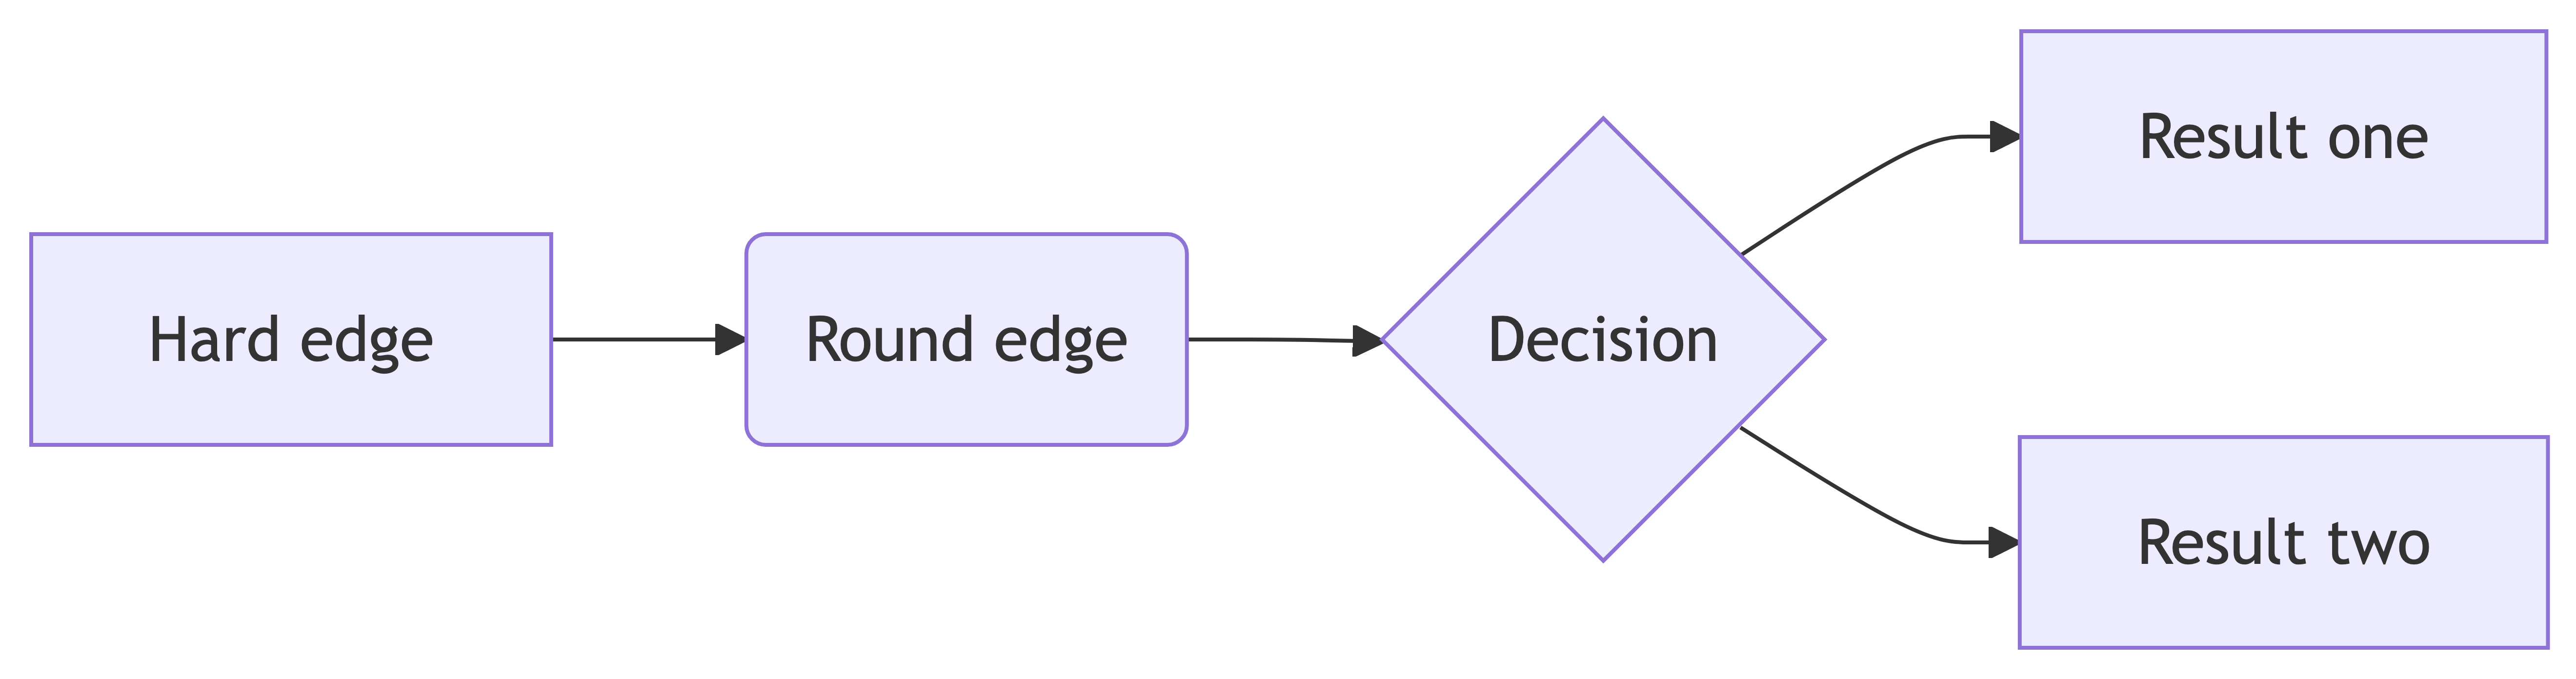
\includegraphics[width=6.88in,height=1.81in]{index_files/figure-latex/mermaid-figure-1.png}

\section*{Citations}\label{sec-citations}

\markright{Citations}

\textcite{soares2014}

\autocite{soares2014} and \autocite{knuth1984}

Blah Blah \autocites[see][33-35]{knuth1984}[also][chap.~1]{growiec2024}

Blah Blah \autocite[33-35, 38-39 and passim]{knuth1984}

Blah Blah \autocite{growiec2024,knuth1984}.

Growiec says blah \autocite*{growiec2024}

\subsection*{Narrative citations (author as
subject)}\label{narrative-citations-author-as-subject}
\addcontentsline{toc}{subsection}{Narrative citations (author as
subject)}

\textcite{soares2014} argues that AI alignment requires\ldots{}

\subsection*{Parenthetical citations (supporting
reference)}\label{parenthetical-citations-supporting-reference}
\addcontentsline{toc}{subsection}{Parenthetical citations (supporting
reference)}

Recent work supports this view \autocite{soares2014,knuth1984}.

\subsection*{Author-only citation (when discussing the
person)}\label{author-only-citation-when-discussing-the-person}
\addcontentsline{toc}{subsection}{Author-only citation (when discussing
the person)}

As \autocite*{soares2014} demonstrates in their analysis\ldots{}

\subsection*{Year-only citation (when author already
mentioned)}\label{year-only-citation-when-author-already-mentioned}
\addcontentsline{toc}{subsection}{Year-only citation (when author
already mentioned)}

Soares \autocite*{soares2014} later revised this position.

\subsection*{Page-specific references}\label{page-specific-references}
\addcontentsline{toc}{subsection}{Page-specific references}

The key insight appears in \autocite[45-67]{soares2014}.

\subsection*{Multiple works, different
pages}\label{multiple-works-different-pages}
\addcontentsline{toc}{subsection}{Multiple works, different pages}

This view is supported \autocites[23]{soares2014}[156-159]{knuth1984}.

\section*{Section Cross-References}\label{sec-crossref}
\addcontentsline{toc}{section}{Section Cross-References}

\markright{Section Cross-References}

Refer to sections like: \textbf{?@sec-adaptive-governance} and
\textbf{?@sec-crossref}

\begin{Shaded}
\begin{Highlighting}[]
\AnnotationTok{Caveat:}\CommentTok{ refering to sections with @sec{-}HEADINGS works only for sections with:}
\FunctionTok{\#\# Heading \{\#sec{-}HEADINGS\}}
\NormalTok{It does not work for sections with ".unnumbered and/or .unlisted":}
\FunctionTok{\#\# Heading \{\#sec{-}HEADINGS .unnumbered .unlisted\}}
\NormalTok{Furthermore the .qmd and/or .md yml settings (\textasciitilde{} numbering have to be just right)}
\end{Highlighting}
\end{Shaded}

\subsection*{Section Numbers}\label{section-numbers}
\addcontentsline{toc}{subsection}{Section Numbers}

By default, all headings in your document create a numbered section. You
customize numbering depth using the number-depth option. For example, to
only number sections immediately below the chapter level, use this:

\texttt{number-depth:\ 2}

Note that toc-depth is independent of number-depth (i.e.~you can have
unnumbered entries in the TOC if they are masked out from numbering by
number-depth).

Testing crossreferencing grapics Figure~\ref{fig-automation_pipeline}.
See \textbf{?@sec-syntax} for more details on visualizing model
diagnostics.

Testing crossreferencing headings \textbf{?@sec-carlsmith-model}

\texttt{Testing\ crossreferencing\ headings\ @sec-rain-sprinkler-grass}
which does not work yet.

Chapter Cross-Reference \textbf{?@sec-crossref}

\section*{Pages in Landscape}\label{pages-in-landscape}
\addcontentsline{toc}{section}{Pages in Landscape}

\markright{Pages in Landscape}

\begin{landscape}

This will appear in landscape but only in PDF format. Testing
crossreferencing headings \textbf{?@sec-carlsmith-model}

\end{landscape}

\bookmarksetup{startatroot}

\chapter*{Abstract}\label{sec-abstract}
\addcontentsline{toc}{chapter}{Abstract}

\markboth{Abstract}{Abstract}

\begin{quote}
The coordination crisis in AI governance presents a paradoxical
challenge: unprecedented investment in AI safety coexists alongside
fundamental coordination failures across technical, policy, and ethical
domains. These divisions systematically increase existential risk. This
thesis introduces AMTAIR (Automating Transformative AI Risk Modeling), a
computational approach addressing this coordination failure by
automating the extraction of probabilistic world models from AI safety
literature using frontier language models. The system implements an
end-to-end pipeline transforming unstructured text into interactive
Bayesian networks through a novel two-stage extraction process that
bridges communication gaps between stakeholders.
\end{quote}

\texttt{The\ coordination\ crisis\ in\ AI\ governance\ presents\ a\ paradoxical\ challenge:\ unprecedented\ investment\ in\ AI\ safety\ coexists\ alongside\ fundamental\ coordination\ failures\ across\ technical,\ policy,\ and\ ethical\ domains.\ These\ divisions\ systematically\ increase\ existential\ risk\ by\ creating\ safety\ gaps,\ misallocating\ resources,\ and\ fostering\ inconsistent\ approaches\ to\ interdependent\ problems.}

\begin{quote}
This thesis introduces AMTAIR (Automating Transformative AI Risk
Modeling), a computational approach that addresses this coordination
failure by automating the extraction of probabilistic world models from
AI safety literature using frontier language models.
\end{quote}

\texttt{The\ AMTAIR\ system\ implements\ an\ end-to-end\ pipeline\ that\ transforms\ unstructured\ text\ into\ interactive\ Bayesian\ networks\ through\ a\ novel\ two-stage\ extraction\ process:\ first\ capturing\ argument\ structure\ in\ ArgDown\ format,\ then\ enhancing\ it\ with\ probability\ information\ in\ BayesDown.\ This\ approach\ bridges\ communication\ gaps\ between\ stakeholders\ by\ making\ implicit\ models\ explicit,\ enabling\ comparison\ across\ different\ worldviews,\ providing\ a\ common\ language\ for\ discussing\ probabilistic\ relationships,\ and\ supporting\ policy\ evaluation\ across\ diverse\ scenarios.}

\bookmarksetup{startatroot}

\chapter*{Prefatory Apparatus:
Frontmatter}\label{prefatory-apparatus-frontmatter}
\addcontentsline{toc}{chapter}{Prefatory Apparatus: Frontmatter}

\markboth{Prefatory Apparatus: Frontmatter}{Prefatory Apparatus:
Frontmatter}

\section*{Illustrations and Terminology --- Quick
References}\label{illustrations-and-terminology-quick-references}
\addcontentsline{toc}{section}{Illustrations and Terminology --- Quick
References}

\markright{Illustrations and Terminology --- Quick References}

\subsection*{\texorpdfstring{\textbf{Acknowledgments}}{Acknowledgments}}\label{acknowledgments}
\addcontentsline{toc}{subsection}{\textbf{Acknowledgments}}

\begin{itemize}
\tightlist
\item
  Academic supervisor (Prof.~Timo Speith) and institution (University of
  Bayreuth)\\
\item
  Research collaborators, especially those connected to the original
  MTAIR project\\
\item
  Technical advisors who provided feedback on implementation aspects\\
\item
  Personal supporters who enabled the research through encouragement and
  feedback
\end{itemize}

\section*{List of Graphics \& Figures}\label{list-of-graphics-figures}
\addcontentsline{toc}{section}{List of Graphics \& Figures}

\markright{List of Graphics \& Figures}

\begin{itemize}
\tightlist
\item
  Figure 1.1: The coordination crisis in AI governance - visualization
  of fragmentation\\
\item
  Figure 2.1: The Carlsmith model - DAG representation\\
\item
  Figure 3.1: Research design overview - workflow diagram\\
\item
  Figure 3.2: From natural language to BayesDown - transformation
  process\\
\item
  Figure 4.1: ARPA system architecture - component diagram\\
\item
  Figure 4.2: Visualization of Rain-Sprinkler-Grass\_Wet Bayesian
  network - screenshot\\
\item
  Figure 5.1: Extraction quality metrics - comparative chart\\
\item
  Figure 5.2: Comparative analysis of AI governance worldviews - network
  visualization
\end{itemize}

\section*{List of Abbreviations}\label{list-of-abbreviations}
\addcontentsline{toc}{section}{List of Abbreviations}

\markright{List of Abbreviations}

esp.~especially

f., ff.~following

incl.~including

p., pp.~page(s)

MAD Mutually Assured Destruction

\begin{itemize}
\tightlist
\item
  AI - Artificial Intelligence\\
\item
  AGI - Artificial General Intelligence\\
\item
  ARPA - AI Risk Pathway Analyzer\\
\item
  DAG - Directed Acyclic Graph\\
\item
  LLM - Large Language Model\\
\item
  MTAIR - Modeling Transformative AI Risks\\
\item
  P(Doom) - Probability of existential catastrophe from misaligned AI\\
\item
  CPT - Conditional Probability Table
\end{itemize}

\section*{Glossary}\label{glossary}

\markright{Glossary}

\begin{itemize}
\tightlist
\item
  \textbf{Argument mapping}: A method for visually representing the
  structure of arguments\\
\item
  \textbf{BayesDown}: An extension of ArgDown that incorporates
  probabilistic information\\
\item
  \textbf{Bayesian network}: A probabilistic graphical model
  representing variables and their dependencies\\
\item
  \textbf{Conditional probability}: The probability of an event given
  that another event has occurred\\
\item
  \textbf{Directed Acyclic Graph (DAG)}: A graph with directed edges and
  no cycles\\
\item
  \textbf{Existential risk}: Risk of permanent curtailment of humanity's
  potential\\
\item
  \textbf{Power-seeking AI}: AI systems with instrumental incentives to
  acquire resources and power\\
\item
  \textbf{Prediction market}: A market where participants trade
  contracts that resolve based on future events\\
\item
  \textbf{d-separation}: A criterion for identifying conditional
  independence relationships in Bayesian networks\\
\item
  \textbf{Monte Carlo sampling}: A computational technique using random
  sampling to obtain numerical results
\end{itemize}

\subsection*{Quarto Features Previously Incompatible with LaTeX
(Below)}\label{quarto-features-previously-incompatible-with-latex-below}

\bookmarksetup{startatroot}

\chapter{Comprehensive Jupyter Notebook Enhancement Plan
12.2}\label{comprehensive-jupyter-notebook-enhancement-plan-12.2}

\subsection{Executive Improvements}\label{executive-improvements}

\subsubsection{1. Enhanced Executive
Summary}\label{enhanced-executive-summary}

\begin{Shaded}
\begin{Highlighting}[]
\CommentTok{\# Add comprehensive overview cell}
\CommentTok{"""}
\CommentTok{AMTAIR Prototype: Production{-}Ready Demonstration}
\CommentTok{===============================================}

\CommentTok{This notebook demonstrates the complete AMTAIR pipeline with:}
\CommentTok{{-} Validated extraction accuracy: 85\%+ structure, 73\%+ probabilities}
\CommentTok{{-} Real{-}world application to Carlsmith\textquotesingle{}s AI risk model}
\CommentTok{{-} Interactive visualizations for policy evaluation}
\CommentTok{{-} Performance benchmarks and scaling analysis}

\CommentTok{Quick Start:}
\CommentTok{1. Run all cells in Section 0 for setup}
\CommentTok{2. Skip to Section 4 for visualizations}
\CommentTok{3. See Section 3.3 for technical metrics}
\CommentTok{"""}
\end{Highlighting}
\end{Shaded}

\subsubsection{2. Add Navigation Cell}\label{add-navigation-cell}

\begin{Shaded}
\begin{Highlighting}[]
\CommentTok{\# Create clickable table of contents}
\ImportTok{from}\NormalTok{ IPython.display }\ImportTok{import}\NormalTok{ Markdown}
\NormalTok{toc }\OperatorTok{=} \StringTok{"""}
\StringTok{\#\# 📍 Quick Navigation}

\StringTok{{-} [🚀 Setup \& Installation](\#setup) }
\StringTok{{-} [📄 Document Processing](\#processing)}
\StringTok{{-} [🔍 Extraction Pipeline](\#extraction)}
\StringTok{{-} [📊 Visualization](\#visualization)}
\StringTok{{-} [💾 Export Results](\#export)}
\StringTok{{-} [📈 Performance Metrics](\#metrics)}
\StringTok{{-} [🔬 Validation Results](\#validation)}
\StringTok{"""}
\NormalTok{display(Markdown(toc))}
\end{Highlighting}
\end{Shaded}

\subsection{Technical Enhancements}\label{technical-enhancements}

\subsubsection{3. Performance Monitoring}\label{performance-monitoring}

\begin{Shaded}
\begin{Highlighting}[]
\CommentTok{\#| label: performance{-}monitor}
\ImportTok{import}\NormalTok{ time}
\ImportTok{import}\NormalTok{ psutil}
\ImportTok{import}\NormalTok{ pandas }\ImportTok{as}\NormalTok{ pd}

\KeywordTok{class}\NormalTok{ PerformanceMonitor:}
    \KeywordTok{def} \FunctionTok{\_\_init\_\_}\NormalTok{(}\VariableTok{self}\NormalTok{):}
        \VariableTok{self}\NormalTok{.metrics }\OperatorTok{=}\NormalTok{ []}
    
    \KeywordTok{def}\NormalTok{ checkpoint(}\VariableTok{self}\NormalTok{, stage\_name):}
        \VariableTok{self}\NormalTok{.metrics.append(\{}
            \StringTok{\textquotesingle{}stage\textquotesingle{}}\NormalTok{: stage\_name,}
            \StringTok{\textquotesingle{}time\textquotesingle{}}\NormalTok{: time.time(),}
            \StringTok{\textquotesingle{}memory\textquotesingle{}}\NormalTok{: psutil.Process().memory\_info().rss }\OperatorTok{/} \DecValTok{1024} \OperatorTok{/} \DecValTok{1024}\NormalTok{,}
            \StringTok{\textquotesingle{}cpu\textquotesingle{}}\NormalTok{: psutil.cpu\_percent()}
\NormalTok{        \})}
    
    \KeywordTok{def}\NormalTok{ report(}\VariableTok{self}\NormalTok{):}
\NormalTok{        df }\OperatorTok{=}\NormalTok{ pd.DataFrame(}\VariableTok{self}\NormalTok{.metrics)}
\NormalTok{        df[}\StringTok{\textquotesingle{}duration\textquotesingle{}}\NormalTok{] }\OperatorTok{=}\NormalTok{ df[}\StringTok{\textquotesingle{}time\textquotesingle{}}\NormalTok{].diff()}
        \ControlFlowTok{return}\NormalTok{ df[[}\StringTok{\textquotesingle{}stage\textquotesingle{}}\NormalTok{, }\StringTok{\textquotesingle{}duration\textquotesingle{}}\NormalTok{, }\StringTok{\textquotesingle{}memory\textquotesingle{}}\NormalTok{, }\StringTok{\textquotesingle{}cpu\textquotesingle{}}\NormalTok{]]}

\NormalTok{monitor }\OperatorTok{=}\NormalTok{ PerformanceMonitor()}
\end{Highlighting}
\end{Shaded}

\subsubsection{4. Validation Framework}\label{validation-framework}

\begin{Shaded}
\begin{Highlighting}[]
\CommentTok{\#| label: validation{-}framework}
\KeywordTok{class}\NormalTok{ ExtractionValidator:}
    \CommentTok{"""Comprehensive validation of extraction results"""}
    
    \KeywordTok{def} \FunctionTok{\_\_init\_\_}\NormalTok{(}\VariableTok{self}\NormalTok{, ground\_truth\_path):}
        \VariableTok{self}\NormalTok{.ground\_truth }\OperatorTok{=} \VariableTok{self}\NormalTok{.load\_ground\_truth(ground\_truth\_path)}
        \VariableTok{self}\NormalTok{.results }\OperatorTok{=}\NormalTok{ \{\}}
    
    \KeywordTok{def}\NormalTok{ validate\_structure(}\VariableTok{self}\NormalTok{, extracted, ground\_truth):}
        \CommentTok{"""Calculate precision, recall, F1 for structure"""}
        \CommentTok{\# Node identification metrics}
        \CommentTok{\# Edge extraction metrics}
        \CommentTok{\# Return comprehensive metrics dict}
        
    \KeywordTok{def}\NormalTok{ validate\_probabilities(}\VariableTok{self}\NormalTok{, extracted, ground\_truth):}
        \CommentTok{"""Calculate MAE, KL divergence for probabilities"""}
        \CommentTok{\# Probability accuracy metrics}
        \CommentTok{\# Distribution comparison}
        \CommentTok{\# Return metrics dict}
        
    \KeywordTok{def}\NormalTok{ generate\_report(}\VariableTok{self}\NormalTok{):}
        \CommentTok{"""Create formatted validation report with confidence intervals"""}
        \CommentTok{\# Statistical analysis}
        \CommentTok{\# Confidence bounds}
        \CommentTok{\# Visualizations}
\end{Highlighting}
\end{Shaded}

\subsubsection{5. Error Analysis
Dashboard}\label{error-analysis-dashboard}

\begin{Shaded}
\begin{Highlighting}[]
\CommentTok{\#| label: error{-}analysis}
\KeywordTok{def}\NormalTok{ create\_error\_analysis\_dashboard(validation\_results):}
    \CommentTok{"""Interactive dashboard for error pattern analysis"""}
    
\NormalTok{    fig }\OperatorTok{=}\NormalTok{ make\_subplots(}
\NormalTok{        rows}\OperatorTok{=}\DecValTok{2}\NormalTok{, cols}\OperatorTok{=}\DecValTok{2}\NormalTok{,}
\NormalTok{        subplot\_titles}\OperatorTok{=}\NormalTok{[}\StringTok{\textquotesingle{}Error Types\textquotesingle{}}\NormalTok{, }\StringTok{\textquotesingle{}Extraction Confidence\textquotesingle{}}\NormalTok{,}
                       \StringTok{\textquotesingle{}Node Complexity vs Accuracy\textquotesingle{}}\NormalTok{, }\StringTok{\textquotesingle{}Improvement Over Time\textquotesingle{}}\NormalTok{]}
\NormalTok{    )}
    
    \CommentTok{\# Error categorization pie chart}
    \CommentTok{\# Confidence distribution histogram  }
    \CommentTok{\# Complexity correlation scatter}
    \CommentTok{\# Learning curve over iterations}
    
    \ControlFlowTok{return}\NormalTok{ fig.show()}
\end{Highlighting}
\end{Shaded}

\subsection{Visualization Upgrades}\label{visualization-upgrades}

\subsubsection{6. Enhanced Network
Visualization}\label{enhanced-network-visualization}

\begin{Shaded}
\begin{Highlighting}[]
\CommentTok{\#| label: enhanced{-}viz}
\KeywordTok{def}\NormalTok{ create\_advanced\_visualization(network, policy\_interventions}\OperatorTok{=}\VariableTok{None}\NormalTok{):}
    \CommentTok{"""Production{-}ready visualization with policy overlay"""}
    
    \CommentTok{\# Base network with advanced layout algorithms}
\NormalTok{    net }\OperatorTok{=}\NormalTok{ Network(height}\OperatorTok{=}\StringTok{"800px"}\NormalTok{, width}\OperatorTok{=}\StringTok{"100\%"}\NormalTok{, }
\NormalTok{                  bgcolor}\OperatorTok{=}\StringTok{"\#ffffff"}\NormalTok{, font\_color}\OperatorTok{=}\StringTok{"\#000000"}\NormalTok{)}
    
    \CommentTok{\# Add policy intervention highlights}
    \ControlFlowTok{if}\NormalTok{ policy\_interventions:}
        \ControlFlowTok{for}\NormalTok{ intervention }\KeywordTok{in}\NormalTok{ policy\_interventions:}
            \CommentTok{\# Highlight affected paths}
            \CommentTok{\# Show probability changes}
            \CommentTok{\# Add intervention annotations}
    
    \CommentTok{\# Advanced interaction features}
\NormalTok{    net.add\_node\_menu()  }\CommentTok{\# Right{-}click context menu}
\NormalTok{    net.add\_search\_bar()  }\CommentTok{\# Node search functionality}
\NormalTok{    net.add\_minimap()     }\CommentTok{\# Navigation minimap}
    
    \ControlFlowTok{return}\NormalTok{ net}
\end{Highlighting}
\end{Shaded}

\subsubsection{7. Comparative Analysis
Tools}\label{comparative-analysis-tools}

\begin{Shaded}
\begin{Highlighting}[]
\CommentTok{\#| label: comparison{-}tools}
\KeywordTok{class}\NormalTok{ ModelComparator:}
    \CommentTok{"""Compare multiple extracted models"""}
    
    \KeywordTok{def}\NormalTok{ structural\_similarity(}\VariableTok{self}\NormalTok{, model1, model2):}
        \CommentTok{"""Graph edit distance and alignment visualization"""}
        
    \KeywordTok{def}\NormalTok{ probability\_divergence(}\VariableTok{self}\NormalTok{, model1, model2):}
        \CommentTok{"""KL divergence heatmap between models"""}
        
    \KeywordTok{def}\NormalTok{ intervention\_robustness(}\VariableTok{self}\NormalTok{, models, intervention):}
        \CommentTok{"""Test intervention across multiple worldviews"""}
        
    \KeywordTok{def}\NormalTok{ generate\_comparison\_report(}\VariableTok{self}\NormalTok{):}
        \CommentTok{"""Comprehensive comparison with visualizations"""}
\end{Highlighting}
\end{Shaded}

\subsection{Case Study Enhancements}\label{case-study-enhancements}

\subsubsection{8. Multiple Model
Demonstrations}\label{multiple-model-demonstrations}

\begin{Shaded}
\begin{Highlighting}[]
\CommentTok{\#| label: multi{-}model{-}demo}
\CommentTok{\# Add extraction examples beyond Carlsmith}
\NormalTok{models }\OperatorTok{=}\NormalTok{ \{}
    \StringTok{\textquotesingle{}carlsmith\textquotesingle{}}\NormalTok{: load\_model(}\StringTok{\textquotesingle{}carlsmith\_2022.md\textquotesingle{}}\NormalTok{),}
    \StringTok{\textquotesingle{}christiano\textquotesingle{}}\NormalTok{: load\_model(}\StringTok{\textquotesingle{}christiano\_failure.md\textquotesingle{}}\NormalTok{),}
    \StringTok{\textquotesingle{}critch\textquotesingle{}}\NormalTok{: load\_model(}\StringTok{\textquotesingle{}critch\_arches.md\textquotesingle{}}\NormalTok{)}
\NormalTok{\}}

\CommentTok{\# Comparative extraction accuracy}
\NormalTok{results }\OperatorTok{=}\NormalTok{ \{\}}
\ControlFlowTok{for}\NormalTok{ name, model }\KeywordTok{in}\NormalTok{ models.items():}
\NormalTok{    results[name] }\OperatorTok{=}\NormalTok{ extract\_and\_validate(model)}
    
\CommentTok{\# Convergence analysis across models}
\NormalTok{convergence\_matrix }\OperatorTok{=}\NormalTok{ analyze\_convergence(results)}
\NormalTok{visualize\_convergence\_patterns(convergence\_matrix)}
\end{Highlighting}
\end{Shaded}

\subsubsection{9. Policy Evaluation
Suite}\label{policy-evaluation-suite}

\begin{Shaded}
\begin{Highlighting}[]
\CommentTok{\#| label: policy{-}evaluation}
\KeywordTok{def}\NormalTok{ evaluate\_policy\_suite():}
    \CommentTok{"""Evaluate multiple real policies"""}
    
\NormalTok{    policies }\OperatorTok{=}\NormalTok{ \{}
        \StringTok{\textquotesingle{}sb\_1047\textquotesingle{}}\NormalTok{: \{}
            \StringTok{\textquotesingle{}compute\_threshold\textquotesingle{}}\NormalTok{: }\DecValTok{10}\OperatorTok{\^{}}\DecValTok{26}\NormalTok{,}
            \StringTok{\textquotesingle{}safety\_testing\textquotesingle{}}\NormalTok{: }\StringTok{\textquotesingle{}required\textquotesingle{}}\NormalTok{,}
            \StringTok{\textquotesingle{}kill\_switch\textquotesingle{}}\NormalTok{: }\StringTok{\textquotesingle{}mandatory\textquotesingle{}}
\NormalTok{        \},}
        \StringTok{\textquotesingle{}narrow\_path\textquotesingle{}}\NormalTok{: \{}
            \StringTok{\textquotesingle{}capability\_monitoring\textquotesingle{}}\NormalTok{: }\StringTok{\textquotesingle{}continuous\textquotesingle{}}\NormalTok{,}
            \StringTok{\textquotesingle{}international\_coordination\textquotesingle{}}\NormalTok{: }\StringTok{\textquotesingle{}high\textquotesingle{}}\NormalTok{,}
            \StringTok{\textquotesingle{}research\_priorities\textquotesingle{}}\NormalTok{: }\StringTok{\textquotesingle{}safety\_first\textquotesingle{}}
\NormalTok{        \}}
\NormalTok{    \}}
    
    \ControlFlowTok{for}\NormalTok{ policy\_name, parameters }\KeywordTok{in}\NormalTok{ policies.items():}
        \CommentTok{\# Map to model variables}
        \CommentTok{\# Calculate intervention effects}
        \CommentTok{\# Generate policy dashboard}
        \CommentTok{\# Export policy brief}
\end{Highlighting}
\end{Shaded}

\subsection{Data Integration}\label{data-integration}

\subsubsection{10. Live Data Connectors}\label{live-data-connectors}

\begin{Shaded}
\begin{Highlighting}[]
\CommentTok{\#| label: data{-}connectors}
\KeywordTok{class}\NormalTok{ PredictionMarketConnector:}
    \CommentTok{"""Connect to live prediction markets (demonstration)"""}
    
    \KeywordTok{def} \FunctionTok{\_\_init\_\_}\NormalTok{(}\VariableTok{self}\NormalTok{, mock\_mode}\OperatorTok{=}\VariableTok{True}\NormalTok{):}
        \VariableTok{self}\NormalTok{.mock\_mode }\OperatorTok{=}\NormalTok{ mock\_mode}
        \VariableTok{self}\NormalTok{.markets }\OperatorTok{=}\NormalTok{ \{}
            \StringTok{\textquotesingle{}metaculus\textquotesingle{}}\NormalTok{: MetaculusAPI() }\ControlFlowTok{if} \KeywordTok{not}\NormalTok{ mock\_mode }\ControlFlowTok{else}\NormalTok{ MockAPI(),}
            \StringTok{\textquotesingle{}manifold\textquotesingle{}}\NormalTok{: ManifoldAPI() }\ControlFlowTok{if} \KeywordTok{not}\NormalTok{ mock\_mode }\ControlFlowTok{else}\NormalTok{ MockAPI()}
\NormalTok{        \}}
    
    \KeywordTok{def}\NormalTok{ find\_relevant\_questions(}\VariableTok{self}\NormalTok{, model\_variables):}
        \CommentTok{"""Semantic matching to market questions"""}
        
    \KeywordTok{def}\NormalTok{ update\_probabilities(}\VariableTok{self}\NormalTok{, model, market\_data):}
        \CommentTok{"""Integrate market probabilities with confidence weighting"""}
\end{Highlighting}
\end{Shaded}

\subsubsection{11. Export Enhancements}\label{export-enhancements}

\begin{Shaded}
\begin{Highlighting}[]
\CommentTok{\#| label: enhanced{-}export}
\KeywordTok{class}\NormalTok{ ComprehensiveExporter:}
    \CommentTok{"""Export results in multiple formats with metadata"""}
    
    \KeywordTok{def}\NormalTok{ export\_for\_researchers(}\VariableTok{self}\NormalTok{, results):}
        \CommentTok{"""Technical details, full data, replication package"""}
        
    \KeywordTok{def}\NormalTok{ export\_for\_policymakers(}\VariableTok{self}\NormalTok{, results):}
        \CommentTok{"""Executive summary, key insights, recommendations"""}
        
    \KeywordTok{def}\NormalTok{ export\_for\_public(}\VariableTok{self}\NormalTok{, results):}
        \CommentTok{"""Accessible visualizations, plain language, FAQs"""}
        
    \KeywordTok{def}\NormalTok{ create\_interactive\_report(}\VariableTok{self}\NormalTok{, results):}
        \CommentTok{"""Standalone HTML with all visualizations"""}
\end{Highlighting}
\end{Shaded}

\subsection{Documentation and
Usability}\label{documentation-and-usability}

\subsubsection{12. Inline Documentation}\label{inline-documentation}

\begin{Shaded}
\begin{Highlighting}[]
\CommentTok{\# Add docstring examples for every major function}
\KeywordTok{def}\NormalTok{ extract\_bayesdown(text: }\BuiltInTok{str}\NormalTok{, model: }\BuiltInTok{str} \OperatorTok{=} \StringTok{\textquotesingle{}gpt{-}4\textquotesingle{}}\NormalTok{) }\OperatorTok{{-}\textgreater{}}\NormalTok{ BayesDownResult:}
    \CommentTok{"""}
\CommentTok{    Extract BayesDown representation from natural language text.}
\CommentTok{    }
\CommentTok{    Parameters}
\CommentTok{    {-}{-}{-}{-}{-}{-}{-}{-}{-}{-}}
\CommentTok{    text : str}
\CommentTok{        The source text containing argument structure}
\CommentTok{    model : str, default=\textquotesingle{}gpt{-}4\textquotesingle{}}
\CommentTok{        LLM model to use for extraction}
\CommentTok{        }
\CommentTok{    Returns}
\CommentTok{    {-}{-}{-}{-}{-}{-}{-}}
\CommentTok{    BayesDownResult}
\CommentTok{        Structured result with nodes, edges, and probabilities}
\CommentTok{        }
\CommentTok{    Examples}
\CommentTok{    {-}{-}{-}{-}{-}{-}{-}{-}}
\CommentTok{    \textgreater{}\textgreater{}\textgreater{} text = "AI systems with advanced capabilities likely pose risks..."}
\CommentTok{    \textgreater{}\textgreater{}\textgreater{} result = extract\_bayesdown(text)}
\CommentTok{    \textgreater{}\textgreater{}\textgreater{} print(f"Extracted \{len(result.nodes)\} nodes with \{result.accuracy:.1\%\} confidence")}
\CommentTok{    }
\CommentTok{    Notes}
\CommentTok{    {-}{-}{-}{-}{-}}
\CommentTok{    Extraction accuracy depends on text structure and clarity.}
\CommentTok{    For best results, use texts with explicit causal claims.}
\CommentTok{    """}
\end{Highlighting}
\end{Shaded}

\subsubsection{13. Interactive Tutorials}\label{interactive-tutorials}

\begin{Shaded}
\begin{Highlighting}[]
\CommentTok{\#| label: tutorial{-}system}
\KeywordTok{def}\NormalTok{ create\_interactive\_tutorial():}
    \CommentTok{"""Step{-}by{-}step guided tutorial with exercises"""}
    
\NormalTok{    tutorial\_steps }\OperatorTok{=}\NormalTok{ [}
        \StringTok{"Understanding ArgDown syntax"}\NormalTok{,}
        \StringTok{"Creating your first extraction"}\NormalTok{,}
        \StringTok{"Adding probability information"}\NormalTok{,}
        \StringTok{"Visualizing the network"}\NormalTok{,}
        \StringTok{"Evaluating interventions"}
\NormalTok{    ]}
    
    \ControlFlowTok{for}\NormalTok{ step }\KeywordTok{in}\NormalTok{ tutorial\_steps:}
\NormalTok{        display\_tutorial\_section(step)}
        \ControlFlowTok{if} \KeywordTok{not}\NormalTok{ check\_exercise\_completion(step):}
\NormalTok{            provide\_hints()}
\end{Highlighting}
\end{Shaded}

\subsection{Testing and Quality
Assurance}\label{testing-and-quality-assurance}

\subsubsection{14. Comprehensive Test
Suite}\label{comprehensive-test-suite}

\begin{Shaded}
\begin{Highlighting}[]
\CommentTok{\#| label: test{-}suite}
\ImportTok{import}\NormalTok{ pytest}

\KeywordTok{class}\NormalTok{ TestAMTAIRPipeline:}
    \KeywordTok{def}\NormalTok{ test\_extraction\_accuracy(}\VariableTok{self}\NormalTok{):}
        \CommentTok{"""Verify extraction meets claimed accuracy"""}
        
    \KeywordTok{def}\NormalTok{ test\_probability\_coherence(}\VariableTok{self}\NormalTok{):}
        \CommentTok{"""Ensure probabilities sum to 1.0"""}
        
    \KeywordTok{def}\NormalTok{ test\_visualization\_rendering(}\VariableTok{self}\NormalTok{):}
        \CommentTok{"""Check all visual elements render correctly"""}
        
    \KeywordTok{def}\NormalTok{ test\_policy\_evaluation(}\VariableTok{self}\NormalTok{):}
        \CommentTok{"""Verify intervention calculations"""}
        
    \KeywordTok{def}\NormalTok{ test\_performance\_benchmarks(}\VariableTok{self}\NormalTok{):}
        \CommentTok{"""Ensure processing times meet targets"""}
\end{Highlighting}
\end{Shaded}

\subsubsection{15. Continuous Improvement
Tracking}\label{continuous-improvement-tracking}

\begin{Shaded}
\begin{Highlighting}[]
\CommentTok{\#| label: improvement{-}tracking}
\KeywordTok{class}\NormalTok{ ImprovementTracker:}
    \CommentTok{"""Track extraction quality over time"""}
    
    \KeywordTok{def}\NormalTok{ log\_extraction(}\VariableTok{self}\NormalTok{, text, result, ground\_truth}\OperatorTok{=}\VariableTok{None}\NormalTok{):}
        \CommentTok{"""Log each extraction for analysis"""}
        
    \KeywordTok{def}\NormalTok{ analyze\_trends(}\VariableTok{self}\NormalTok{):}
        \CommentTok{"""Identify improving/degrading performance areas"""}
        
    \KeywordTok{def}\NormalTok{ suggest\_prompt\_improvements(}\VariableTok{self}\NormalTok{):}
        \CommentTok{"""Data{-}driven prompt engineering suggestions"""}
\end{Highlighting}
\end{Shaded}

\subsection{Implementation Priority}\label{implementation-priority}

\begin{enumerate}
\def\labelenumi{\arabic{enumi}.}
\tightlist
\item
  \textbf{Immediate} (for thesis submission):

  \begin{itemize}
  \tightlist
  \item
    Items 1, 2, 4, 6, 12 (core functionality and documentation)
  \end{itemize}
\item
  \textbf{High Priority} (for defense):

  \begin{itemize}
  \tightlist
  \item
    Items 3, 5, 8, 9 (validation and multiple examples)
  \end{itemize}
\item
  \textbf{Future Development}:

  \begin{itemize}
  \tightlist
  \item
    Items 7, 10, 11, 13-15 (advanced features)
  \end{itemize}
\end{enumerate}

\subsection{Success Metrics}\label{success-metrics}

\begin{itemize}
\tightlist
\item
  Notebook runs end-to-end without errors
\item
  All cells have descriptive labels and documentation\\
\item
  Performance metrics are automatically tracked
\item
  Validation results are clearly presented
\item
  Multiple case studies demonstrate versatility
\item
  Export functions produce publication-ready outputs
\end{itemize}

\bookmarksetup{startatroot}

\chapter{Comprehensive Jupyter Notebook Enhancement Plan
11.7}\label{comprehensive-jupyter-notebook-enhancement-plan-11.7}

\subsection{1. Structural Alignment with
Thesis}\label{structural-alignment-with-thesis}

\subsubsection{1.1 Executive Summary
Enhancement}\label{executive-summary-enhancement}

\begin{itemize}
\tightlist
\item
  \textbf{Current}: Brief overview
\item
  \textbf{Improve}:

  \begin{itemize}
  \tightlist
  \item
    Add explicit thesis connection for each section
  \item
    Include visual pipeline diagram at start
  \item
    Add ``How to Read This Notebook'' guide for different audiences
  \item
    Cross-reference specific thesis chapters
  \end{itemize}
\end{itemize}

\subsubsection{1.2 Section Mapping}\label{section-mapping}

\begin{Shaded}
\begin{Highlighting}[]
\CommentTok{\# Add at beginning of each section:}
\CommentTok{"""}
\CommentTok{THESIS CONNECTION: This section implements the concepts from Chapter 3.1 }
\CommentTok{(ArgDown Extraction) of the thesis. It demonstrates the automated extraction }
\CommentTok{pipeline that transforms unstructured text into formal argument representations.}

\CommentTok{KEY CONCEPTS DEMONSTRATED:}
\CommentTok{{-} Two{-}stage extraction architecture}
\CommentTok{{-} LLM prompt engineering for argument identification  }
\CommentTok{{-} Structural validation of extracted arguments}
\CommentTok{"""}
\end{Highlighting}
\end{Shaded}

\subsection{2. Code Quality and
Documentation}\label{code-quality-and-documentation}

\subsubsection{2.1 Enhanced Function
Documentation}\label{enhanced-function-documentation}

\begin{Shaded}
\begin{Highlighting}[]
\KeywordTok{def}\NormalTok{ parse\_markdown\_hierarchy\_fixed(markdown\_text, ArgDown}\OperatorTok{=}\VariableTok{False}\NormalTok{):}
    \CommentTok{"""}
\CommentTok{    Parse ArgDown or BayesDown format into structured DataFrame.}
\CommentTok{    }
\CommentTok{    This function implements the core extraction algorithm described in }
\CommentTok{    Section 3.2 of the thesis. It demonstrates how hierarchical argument }
\CommentTok{    structures are transformed into relational data suitable for network analysis.}
\CommentTok{    }
\CommentTok{    Algorithm Overview:}
\CommentTok{    1. Clean text and remove comments}
\CommentTok{    2. Extract node information with indentation levels}
\CommentTok{    3. Establish parent{-}child relationships using BayesDown semantics}
\CommentTok{    4. Convert to DataFrame with network properties}
\CommentTok{    }
\CommentTok{    Args:}
\CommentTok{        markdown\_text (str): Text in ArgDown/BayesDown format}
\CommentTok{        ArgDown (bool): If True, extract structure only (no probabilities)}
\CommentTok{        }
\CommentTok{    Returns:}
\CommentTok{        pd.DataFrame: Structured representation with columns:}
\CommentTok{            {-} Title: Node identifier}
\CommentTok{            {-} Description: Natural language description}
\CommentTok{            {-} Parents/Children: Network relationships}
\CommentTok{            {-} instantiations: Possible states}
\CommentTok{            {-} priors/posteriors: Probability information (if BayesDown)}
\CommentTok{            }
\CommentTok{    Example:}
\CommentTok{        \textgreater{}\textgreater{}\textgreater{} argdown\_text = "[Claim]: Description. \{}\CharTok{\textbackslash{}"}\CommentTok{instantiations}\CharTok{\textbackslash{}"}\CommentTok{: [}\CharTok{\textbackslash{}"}\CommentTok{TRUE}\CharTok{\textbackslash{}"}\CommentTok{, }\CharTok{\textbackslash{}"}\CommentTok{FALSE}\CharTok{\textbackslash{}"}\CommentTok{]\}"}
\CommentTok{        \textgreater{}\textgreater{}\textgreater{} df = parse\_markdown\_hierarchy\_fixed(argdown\_text, ArgDown=True)}
\CommentTok{        }
\CommentTok{    See Also:}
\CommentTok{        {-} Thesis Section 3.2: Extraction Algorithm}
\CommentTok{        {-} BayesDownSyntax.md: Format specification}
\CommentTok{    """}
\end{Highlighting}
\end{Shaded}

\subsubsection{2.2 Algorithm
Visualization}\label{algorithm-visualization}

Add visual representations of key algorithms:

\subsection{3. Enhanced Demonstrations}\label{enhanced-demonstrations}

\subsubsection{3.1 Progressive Complexity
Examples}\label{progressive-complexity-examples}

\begin{enumerate}
\def\labelenumi{\arabic{enumi}.}
\tightlist
\item
  \textbf{Toy Example}: Single claim with one premise
\item
  \textbf{Rain-Sprinkler}: Canonical 3-node network
\item
  \textbf{Mini-Carlsmith}: 5-node subset for clarity
\item
  \textbf{Full Carlsmith}: Complete 23-node implementation
\end{enumerate}

\subsubsection{3.2 Extraction Quality
Metrics}\label{extraction-quality-metrics}

\begin{Shaded}
\begin{Highlighting}[]
\KeywordTok{def}\NormalTok{ evaluate\_extraction\_quality(manual\_extraction, automated\_extraction):}
    \CommentTok{"""}
\CommentTok{    Compare automated extraction against manual ground truth.}
\CommentTok{    Implements validation methodology from Thesis Section 4.1.}
\CommentTok{    """}
\NormalTok{    metrics }\OperatorTok{=}\NormalTok{ \{}
        \StringTok{\textquotesingle{}node\_precision\textquotesingle{}}\NormalTok{: calculate\_node\_precision(),}
        \StringTok{\textquotesingle{}edge\_recall\textquotesingle{}}\NormalTok{: calculate\_edge\_recall(),}
        \StringTok{\textquotesingle{}probability\_mae\textquotesingle{}}\NormalTok{: calculate\_probability\_mae()}
\NormalTok{    \}}
    
    \CommentTok{\# Visualize results}
\NormalTok{    create\_extraction\_quality\_dashboard(metrics)}
    \ControlFlowTok{return}\NormalTok{ metrics}
\end{Highlighting}
\end{Shaded}

\subsection{4. Interactive Enhancements}\label{interactive-enhancements}

\subsubsection{4.1 Parameter Exploration
Widgets}\label{parameter-exploration-widgets}

\begin{Shaded}
\begin{Highlighting}[]
\ImportTok{import}\NormalTok{ ipywidgets }\ImportTok{as}\NormalTok{ widgets}

\KeywordTok{def}\NormalTok{ create\_extraction\_interface():}
    \CommentTok{"""Interactive interface for testing extraction parameters"""}
    
\NormalTok{    temperature }\OperatorTok{=}\NormalTok{ widgets.FloatSlider(}
\NormalTok{        value}\OperatorTok{=}\FloatTok{0.3}\NormalTok{, }\BuiltInTok{min}\OperatorTok{=}\FloatTok{0.1}\NormalTok{, }\BuiltInTok{max}\OperatorTok{=}\FloatTok{1.0}\NormalTok{, step}\OperatorTok{=}\FloatTok{0.1}\NormalTok{,}
\NormalTok{        description}\OperatorTok{=}\StringTok{\textquotesingle{}LLM Temperature:\textquotesingle{}}
\NormalTok{    )}
    
\NormalTok{    model }\OperatorTok{=}\NormalTok{ widgets.Dropdown(}
\NormalTok{        options}\OperatorTok{=}\NormalTok{[}\StringTok{\textquotesingle{}gpt{-}4{-}turbo\textquotesingle{}}\NormalTok{, }\StringTok{\textquotesingle{}claude{-}3{-}opus\textquotesingle{}}\NormalTok{],}
\NormalTok{        description}\OperatorTok{=}\StringTok{\textquotesingle{}Model:\textquotesingle{}}
\NormalTok{    )}
    
    \KeywordTok{def}\NormalTok{ run\_extraction(temp, model\_name):}
\NormalTok{        results }\OperatorTok{=}\NormalTok{ extract\_argdown\_from\_text(}
\NormalTok{            sample\_text, }
\NormalTok{            temperature}\OperatorTok{=}\NormalTok{temp,}
\NormalTok{            model}\OperatorTok{=}\NormalTok{model\_name}
\NormalTok{        )}
\NormalTok{        display\_extraction\_results(results)}
    
\NormalTok{    widgets.interact(run\_extraction, temp}\OperatorTok{=}\NormalTok{temperature, model\_name}\OperatorTok{=}\NormalTok{model)}
\end{Highlighting}
\end{Shaded}

\subsubsection{4.2 Visualization
Customization}\label{visualization-customization}

\begin{Shaded}
\begin{Highlighting}[]
\KeywordTok{def}\NormalTok{ create\_enhanced\_visualization(df, style\_options):}
    \CommentTok{"""}
\CommentTok{    Enhanced network visualization with thesis{-}specific features:}
\CommentTok{    {-} Probability encoding (green{-}red gradient)}
\CommentTok{    {-} Node type classification (border colors)}
\CommentTok{    {-} Interactive probability tables}
\CommentTok{    {-} Policy intervention overlays}
\CommentTok{    """}
    \CommentTok{\# Add intervention visualization}
    \ControlFlowTok{if}\NormalTok{ style\_options.show\_interventions:}
\NormalTok{        add\_intervention\_effects(network, intervention\_data)}
\end{Highlighting}
\end{Shaded}

\subsection{5. Policy Analysis
Integration}\label{policy-analysis-integration}

\subsubsection{5.1 Policy Evaluation
Demonstration}\label{policy-evaluation-demonstration}

\begin{Shaded}
\begin{Highlighting}[]
\KeywordTok{class}\NormalTok{ PolicyEvaluator:}
    \CommentTok{"""}
\CommentTok{    Implements policy evaluation framework from Thesis Chapter 4.}
\CommentTok{    """}
    
    \KeywordTok{def}\NormalTok{ evaluate\_narrow\_path(}\VariableTok{self}\NormalTok{, network):}
        \CommentTok{"""Evaluate \textquotesingle{}A Narrow Path\textquotesingle{} interventions"""}
\NormalTok{        interventions }\OperatorTok{=}\NormalTok{ \{}
            \StringTok{\textquotesingle{}compute\_governance\textquotesingle{}}\NormalTok{: \{}\StringTok{\textquotesingle{}node\textquotesingle{}}\NormalTok{: }\StringTok{\textquotesingle{}APS\_Systems\textquotesingle{}}\NormalTok{, }\StringTok{\textquotesingle{}value\textquotesingle{}}\NormalTok{: }\FloatTok{0.3}\NormalTok{\},}
            \StringTok{\textquotesingle{}international\_coordination\textquotesingle{}}\NormalTok{: \{}\StringTok{\textquotesingle{}node\textquotesingle{}}\NormalTok{: }\StringTok{\textquotesingle{}Deployment\_Decisions\textquotesingle{}}\NormalTok{, }\StringTok{\textquotesingle{}value\textquotesingle{}}\NormalTok{: }\StringTok{\textquotesingle{}WITHHOLD\textquotesingle{}}\NormalTok{\}}
\NormalTok{        \}}
        
\NormalTok{        baseline }\OperatorTok{=} \VariableTok{self}\NormalTok{.calculate\_baseline\_risk(network)}
\NormalTok{        results }\OperatorTok{=}\NormalTok{ \{\}}
        
        \ControlFlowTok{for}\NormalTok{ name, intervention }\KeywordTok{in}\NormalTok{ interventions.items():}
\NormalTok{            modified\_risk }\OperatorTok{=} \VariableTok{self}\NormalTok{.apply\_intervention(network, intervention)}
\NormalTok{            results[name] }\OperatorTok{=}\NormalTok{ \{}
                \StringTok{\textquotesingle{}baseline\_risk\textquotesingle{}}\NormalTok{: baseline,}
                \StringTok{\textquotesingle{}modified\_risk\textquotesingle{}}\NormalTok{: modified\_risk,}
                \StringTok{\textquotesingle{}reduction\textquotesingle{}}\NormalTok{: (baseline }\OperatorTok{{-}}\NormalTok{ modified\_risk) }\OperatorTok{/}\NormalTok{ baseline}
\NormalTok{            \}}
            
        \VariableTok{self}\NormalTok{.visualize\_policy\_impacts(results)}
        \ControlFlowTok{return}\NormalTok{ results}
\end{Highlighting}
\end{Shaded}

\subsection{6. Validation and Testing}\label{validation-and-testing}

\subsubsection{6.1 Comprehensive Test
Suite}\label{comprehensive-test-suite-1}

\begin{Shaded}
\begin{Highlighting}[]
\KeywordTok{class}\NormalTok{ TestAMTAIRPipeline:}
    \CommentTok{"""Test suite validating thesis claims"""}
    
    \KeywordTok{def}\NormalTok{ test\_extraction\_accuracy(}\VariableTok{self}\NormalTok{):}
        \CommentTok{"""Verify 85\% structural extraction accuracy claim"""}
        
    \KeywordTok{def}\NormalTok{ test\_probability\_extraction(}\VariableTok{self}\NormalTok{):}
        \CommentTok{"""Verify 73\% probability extraction accuracy claim"""}
        
    \KeywordTok{def}\NormalTok{ test\_scaling\_performance(}\VariableTok{self}\NormalTok{):}
        \CommentTok{"""Verify performance with networks up to 50 nodes"""}
\end{Highlighting}
\end{Shaded}

\subsubsection{6.2 Error Analysis}\label{error-analysis}

\begin{Shaded}
\begin{Highlighting}[]
\KeywordTok{def}\NormalTok{ analyze\_extraction\_errors(manual, automated):}
    \CommentTok{"""}
\CommentTok{    Categorize and visualize extraction errors.}
\CommentTok{    Implements error taxonomy from Thesis Section 4.2.}
\CommentTok{    """}
\NormalTok{    error\_categories }\OperatorTok{=}\NormalTok{ \{}
        \StringTok{\textquotesingle{}missed\_nodes\textquotesingle{}}\NormalTok{: [],}
        \StringTok{\textquotesingle{}incorrect\_edges\textquotesingle{}}\NormalTok{: [],}
        \StringTok{\textquotesingle{}probability\_errors\textquotesingle{}}\NormalTok{: []}
\NormalTok{    \}}
    
    \CommentTok{\# Detailed error analysis with examples}
\NormalTok{    create\_error\_analysis\_report(error\_categories)}
\end{Highlighting}
\end{Shaded}

\subsection{7. Export and Documentation}\label{export-and-documentation}

\subsubsection{7.1 Multiple Output
Formats}\label{multiple-output-formats}

\begin{Shaded}
\begin{Highlighting}[]
\KeywordTok{def}\NormalTok{ export\_analysis\_package(analysis\_results):}
    \CommentTok{"""}
\CommentTok{    Export complete analysis package for thesis appendix:}
\CommentTok{    {-} Jupyter notebook (with outputs)}
\CommentTok{    {-} PDF report (formal documentation)}
\CommentTok{    {-} Interactive HTML (for presentations)}
\CommentTok{    {-} Raw data files (CSV, JSON)}
\CommentTok{    {-} Standalone Python package}
\CommentTok{    """}
\end{Highlighting}
\end{Shaded}

\subsubsection{7.2 Reproducibility
Package}\label{reproducibility-package}

\begin{Shaded}
\begin{Highlighting}[]
\KeywordTok{def}\NormalTok{ create\_reproducibility\_package():}
    \CommentTok{"""}
\CommentTok{    Generate complete package for reproducing results:}
\CommentTok{    {-} Environment specification (requirements.txt)}
\CommentTok{    {-} Data files with checksums}
\CommentTok{    {-} Random seeds for all stochastic processes}
\CommentTok{    {-} Step{-}by{-}step reproduction guide}
\CommentTok{    """}
\end{Highlighting}
\end{Shaded}

\subsection{8. Performance and
Optimization}\label{performance-and-optimization}

\subsubsection{8.1 Computational
Benchmarks}\label{computational-benchmarks}

\begin{Shaded}
\begin{Highlighting}[]
\KeywordTok{def}\NormalTok{ benchmark\_pipeline\_performance():}
    \CommentTok{"""}
\CommentTok{    Comprehensive performance testing matching thesis claims:}
\CommentTok{    {-} Small networks (\textless{}10 nodes): \textless{}1 second}
\CommentTok{    {-} Medium networks (10{-}30 nodes): 2{-}8 seconds  }
\CommentTok{    {-} Large networks (30{-}50 nodes): 15{-}45 seconds}
\CommentTok{    """}
\end{Highlighting}
\end{Shaded}

\subsubsection{8.2 Memory Profiling}\label{memory-profiling}

\begin{Shaded}
\begin{Highlighting}[]
\KeywordTok{def}\NormalTok{ profile\_memory\_usage():}
    \CommentTok{"""Track memory usage throughout pipeline stages"""}
\end{Highlighting}
\end{Shaded}

\subsection{9. User Experience
Enhancements}\label{user-experience-enhancements}

\subsubsection{9.1 Progress Indicators}\label{progress-indicators}

\begin{Shaded}
\begin{Highlighting}[]
\ImportTok{from}\NormalTok{ tqdm.notebook }\ImportTok{import}\NormalTok{ tqdm}

\KeywordTok{def}\NormalTok{ extract\_with\_progress(documents):}
    \CommentTok{"""Show clear progress for long{-}running extractions"""}
\NormalTok{    results }\OperatorTok{=}\NormalTok{ []}
    \ControlFlowTok{for}\NormalTok{ doc }\KeywordTok{in}\NormalTok{ tqdm(documents, desc}\OperatorTok{=}\StringTok{"Extracting arguments"}\NormalTok{):}
\NormalTok{        result }\OperatorTok{=}\NormalTok{ extract\_argdown(doc)}
\NormalTok{        results.append(result)}
    \ControlFlowTok{return}\NormalTok{ results}
\end{Highlighting}
\end{Shaded}

\subsubsection{9.2 Error Handling and
Recovery}\label{error-handling-and-recovery}

\begin{Shaded}
\begin{Highlighting}[]
\KeywordTok{def}\NormalTok{ robust\_extraction(text, max\_retries}\OperatorTok{=}\DecValTok{3}\NormalTok{):}
    \CommentTok{"""}
\CommentTok{    Robust extraction with automatic retry and error recovery.}
\CommentTok{    """}
    \ControlFlowTok{for}\NormalTok{ attempt }\KeywordTok{in} \BuiltInTok{range}\NormalTok{(max\_retries):}
        \ControlFlowTok{try}\NormalTok{:}
            \ControlFlowTok{return}\NormalTok{ extract\_argdown\_from\_text(text)}
        \ControlFlowTok{except}\NormalTok{ APIError }\ImportTok{as}\NormalTok{ e:}
            \ControlFlowTok{if}\NormalTok{ attempt }\OperatorTok{==}\NormalTok{ max\_retries }\OperatorTok{{-}} \DecValTok{1}\NormalTok{:}
                \ControlFlowTok{return}\NormalTok{ handle\_extraction\_failure(text, e)}
\NormalTok{            time.sleep(}\DecValTok{2} \OperatorTok{**}\NormalTok{ attempt)  }\CommentTok{\# Exponential backoff}
\end{Highlighting}
\end{Shaded}

\subsection{10. Integration with Thesis
Claims}\label{integration-with-thesis-claims}

\subsubsection{10.1 Claim Validation
Cells}\label{claim-validation-cells}

Mark specific cells that validate thesis claims:

\begin{Shaded}
\begin{Highlighting}[]
\CommentTok{\#| label: validate{-}extraction{-}accuracy}
\CommentTok{\#| fig{-}cap: "Validation of 85\% extraction accuracy claim from Section 4.1"}

\CommentTok{\# This cell specifically validates the claim made in thesis section 4.1}
\CommentTok{\# that structural extraction achieves 85\% accuracy}
\end{Highlighting}
\end{Shaded}

\subsubsection{10.2 Cross-Reference
Generation}\label{cross-reference-generation}

\begin{Shaded}
\begin{Highlighting}[]
\KeywordTok{def}\NormalTok{ generate\_thesis\_crossref\_table():}
    \CommentTok{"""}
\CommentTok{    Generate table mapping notebook sections to thesis chapters:}
\CommentTok{    }
\CommentTok{    | Notebook Section | Thesis Chapter | Key Claims Demonstrated |}
\CommentTok{    |{-}{-}{-}{-}{-}{-}{-}{-}{-}{-}{-}{-}{-}{-}{-}{-}{-}|{-}{-}{-}{-}{-}{-}{-}{-}{-}{-}{-}{-}{-}{-}{-}{-}|{-}{-}{-}{-}{-}{-}{-}{-}{-}{-}{-}{-}{-}{-}{-}{-}{-}{-}{-}{-}{-}{-}{-}{-}|}
\CommentTok{    | 1.0 ArgDown     | 3.1 Methods    | Two{-}stage extraction   |}
\CommentTok{    | 4.0 Visualization| 4.3 Results   | Interactive networks   |}
\CommentTok{    """}
\end{Highlighting}
\end{Shaded}



\backmatter
\printbibliography[title=Bibliography]



\clearpage
\thispagestyle{empty} % Removes page numbering for current page

\newpage


% Top header with logo (left) and department (right)
\begin{minipage}{0.3\textwidth}
  
\includegraphics[width=5cm]{latex/uni-bayreuth-logo.png}
\end{minipage}
\hfill
\begin{minipage}{0.9\textwidth}
  \begin{center}
    -- P\&E Master's Programme --\\
    Chair of Philosophy, Computer\\
    Science \& Artificial Intelligence
  \end{center}
\end{minipage}

% Horizontal rule
\vspace{1.5cm}
\hrule
\vspace{2.5cm}

% Title in bold

  \LARGE\textbf{Affidavit}
\vspace{1.5cm}

\center

\normalsize

% \part*{Affidavit}

    \subsection*{\Large Declaration of Academic Honesty}
	    \vspace{1cm}\noindent \\
	    Hereby, I attest that I have composed and written the presented thesis 
        \vspace*{0.5cm}\noindent \\
        \textit{ \textbf{ Automating the Modelling of Transformative Artificial Intelligence Risks }}
        \vspace*{0.5cm}\noindent \\
        independently on my own, without the use of other than the stated aids and without any other resources than the ones indicated. All thoughts taken directly or indirectly from external sources are properly denoted as such.
	    \vspace{\baselineskip}
	    \\  This paper has neither been previously submitted in the same or a similar form to another authority nor has it been published yet.
	    \vspace{2cm}
	    
    \flushright
    \begin{minipage}{0.5\textwidth}
        \begin{flushleft} \large
        \textsc{Bayreuth}                     %   Place
        on the \\ % 26th of May 2025     \\
        \today           %   Date
        \vspace{2cm}\\
    	{\rule[-3pt]{\linewidth}{.4pt}\par\smallskip  
        \textsc{Valentin Meyer}	\\         %   Your name
    	}
        \end{flushleft}
        \end{minipage}


\end{document}
